\documentclass{article}

\usepackage{graphicx}

\renewcommand{\labelenumii}{\theenumii}
\renewcommand{\theenumii}{\theenumi.\arabic{enumii}.}
\renewcommand{\theenumiii}{\theenumii\arabic{enumiii}.}


\begin{document}
\begin{figure}[t!]
	
\includegraphics[width= \linewidth]{PolimiLogo.png}
	\begin{center}
	Politecnico di Milano\\[4pt]
	AA 2018-2019  \\[4pt]
	Computer Science and Engineering \\[4pt]
	\begin{large}
	Software Engineering 2 Project
	\end{large}
	\end{center}
\end{figure}
\begin{flushright}
\begin{large}
Dalle Rive Fabio - 920082 \\[4pt]
Di Giacomantonio Marco - 846515 \\[4pt]
\end{large}
\end{flushright}
\newpage
\textbf{Table of Contents}
	\begin{enumerate}
			\item Introduction
			\begin{enumerate}
				\item Purpose
				\item Scope
				\begin{enumerate}
					\item Description of the given problem
					\item Goals
				\end{enumerate}
				\item Definitions, Acronyms, Abbreviations
				\begin{enumerate}
					\item Definitions
					\item Acronyms
					\item Abbreviations
				\end{enumerate}
				\item Document structure
			\end{enumerate}
			\item Overall Description
			\begin{enumerate}
				\item Product perspective
				\item Product functions
				\begin{enumerate}
					\item 
				\end{enumerate}
				\item User characteristics
				\item Assumptions, dependencies and constraints
				\begin{enumerate}
					\item Domain assumptions
				\end{enumerate}
			\end{enumerate}
			\item Specific requirements
			\begin{enumerate}
				\item External interface requirements	
				\begin{enumerate}
					\item Users interfaces
					\item Hardware interfaces
					\item Software interfaces
					\item Communication interfaces
				\end{enumerate}
				\item Scenarios
				\begin{enumerate}
					\item
				\end{enumerate}
				\item Functional requirements
				\begin{enumerate}
					\item Use case diagram
					\item Sequence diagram
				\end{enumerate}
				\item Performance requirements
				\item Design Constraints
				\begin{enumerate}
					\item Standard compliance
					\item Hardware limitation
					\item Other constraint
				\end{enumerate}
				\newpage
				\item Software system attributes
				\begin{enumerate}
					\item Reliability
					\item Security
					\item Maintainability
					\item Compatibility
				\end{enumerate}
			\end{enumerate}
			\item Formal Analysis Using Alloy
			\begin{enumerate}
				\item Alloy model
				\item World generated
				\item Alloy results
			\end{enumerate}
			\item Effort Spent
			\item Resources
	\end{enumerate}
	\newpage
\section{Introduction}
\subsection{Purpose}
The purpose of this project is to build a system, called Data4Help, that allows third parties to monitor the position and health status of users. The data are collected by TrackMe, the company that wants to develop Data4Help, and are shared with other companies which are interested in those data.
Furthermore, TrackMe wants to develop AutomatedSOS, a system build on top of Data4Help. AutomatedSOS is a service designed for elderly people, it is able to intervene by calling an ambulance if the health parameters of the user are below some fixed thresholds.
\subsection{Scope}
\subsubsection{Description of the given problem}
TrackMe is a company that wants to develop a software-based service allowing third parties to monitor the location and health status of users. This service is called Data4Help. The service supports the registration of the visitors who, by registering, allow TrackMe to acquire their data. Also it supports the registration of third parties. After registration, these third parties can request: 
\begin{itemize}
	\item Access to the data of some specific user.
	\item Access to anonymized data of groups of users.
\end{itemize}
TrackMe also wants to develop a non-intrusive SOS service for elderly people, called AutomatedSOS. AutomatedSOS is build on top of Data4Help. This service is designed to monitor health status of users and to send an ambulance to the location of the user if some parameters are below some specified thresholds. 
\subsubsection{Goals}
\begin{itemize}
	\item {[G1]} Visitor can become User after providing credentials.
	\item {[G2]} User can accept or reject the request of access to his data formulated by companies.
	\item {[G3]} If user's parameters are below specified thresholds, an ambulance is called within 5 seconds. 
	\begin{itemize}
		\item {[G3.1]} Ambulance is required at current user's location. 
	\end{itemize}
	\item {[G4]} Company can sign up as Company to Data4Help and AutomatedSOS. 
	\item {[G5]} Company can be recognized providing a password and vat number.
	\item {[G6]} Company can formulate a request to see anonymized data of a group of users.
	\item {[G7]} Company can formulate a request to see data of a specific user providing his SSN.
	\item {[G8]} Company can see anonymized data of a group of users.
	\item {[G9]} Company can see data of a specific user providing his SSN.
	\item {[G10]} Company can subscribe to users' new data.
	\item {[G11]} Data4Help can anonymise data.
	\item {[G12]} Data4Help can forward companies' requests to users. 
	\item {[G13]} ??? TrackMe able to withdraw a company ????
\end{itemize} 
\subsection{Definitions, Acronyms, Abbreviations}
\subsubsection{Definitions}
\begin{itemize}
	\item\textbf{Visitor:} a person who still has to register to Data4Help and\\ AutomatedSOS.
	\item\textbf{User:} a person who is registered to Data4Help and AutomatedSOS.
	\item\textbf{Third Parties / Companies:} company.
	\item\textbf{Data:} User's monitored data: location + heart rate + calories burned + time spent exercising + step walked 
	\item \textbf{Threshold:} Flexible value related to the biomedical data acquired by the smart watch in which the system-to-be is installed. This value is computed by well-known equation that operate with user's data. It also depends of the kind of activity that a user is doing.  
	\item \textbf{Request:} Formal request that a company issue to Data4Help in order to access data of a single user or a group of users. 
	\item \textbf{Subscribe to data:} A company which is subscribed to user's data or to users group's data, receives the requested data as soon as they are produced.  
	\item \textbf{Pendent user:} A user that a company want to follow but has not answered to the following request yet.
	\item \textbf{Single user request / Following request:} A formal request issued by a company to see the data of a user.
	\item \textbf{Group of users request:} A formal request issued by a company to see the data of a group of users.
\end{itemize}
\subsubsection{Acronyms}
\begin{itemize}
	\item RASD - Required Analysis and Specification Document
	\item GPS - Global Positioning System
	\item SSN - Social Security Number
\end{itemize}
\subsubsection{Abbreviations}
\begin{itemize}
	\item {[Gn]}: n-th goal
	\item {[Dn]}: n-th domain assumption
	\item {[Rn]}: n-th functional requirement
\end{itemize}
\subsection{Document structure}
\begin{description}
	\item [Introduction] gives an introduction to the problem and describe the purpose of Data4Help and AutomatedSOS. It also contains the goals that these systems-to-be must be able to deliver to users and third party companies.
	\item [Overall Description] gives an overview of the functions that the systems-to-be are able to deliver to users and third parties. In this section, users of the systems-to-be, are better identified, i.e. the kind of users that interact with Data4Help and AutomatedSOS. Due to the imprecise nature of natural language used in the specification of the project, a more formal presentation of the assumptions is required. Assumptions used by Data4Help and AutomatedSOS are presented in this section. 
	\item [Specific Requirements]
	\item [Formal Analysis Using Alloy] includes the Alloy model and the discussion of its purpose. Also, a world generated by this model is shown.
	\item [Effort Spent] shows the effort spent by each group member while working on this project.
	\item [Resources] includes the reference documents. 
\end{description}
\section{Overall Description}
\subsection{Product perspective}
Data4Help and AutomatedSOS are intended as a background application that are installed inside a smart watch. The systems-to-be acquire data of the users through the smart watch. The user register himself for Data4Help on the website page that TrackMe provide for this application. Users access to the web page through their Google or Apple account. These accounts are used by TrackMe in order to understand from which devices it will acquire data.
\begin{figure}[h!]
\centering
    \textbf{}\par\medskip
	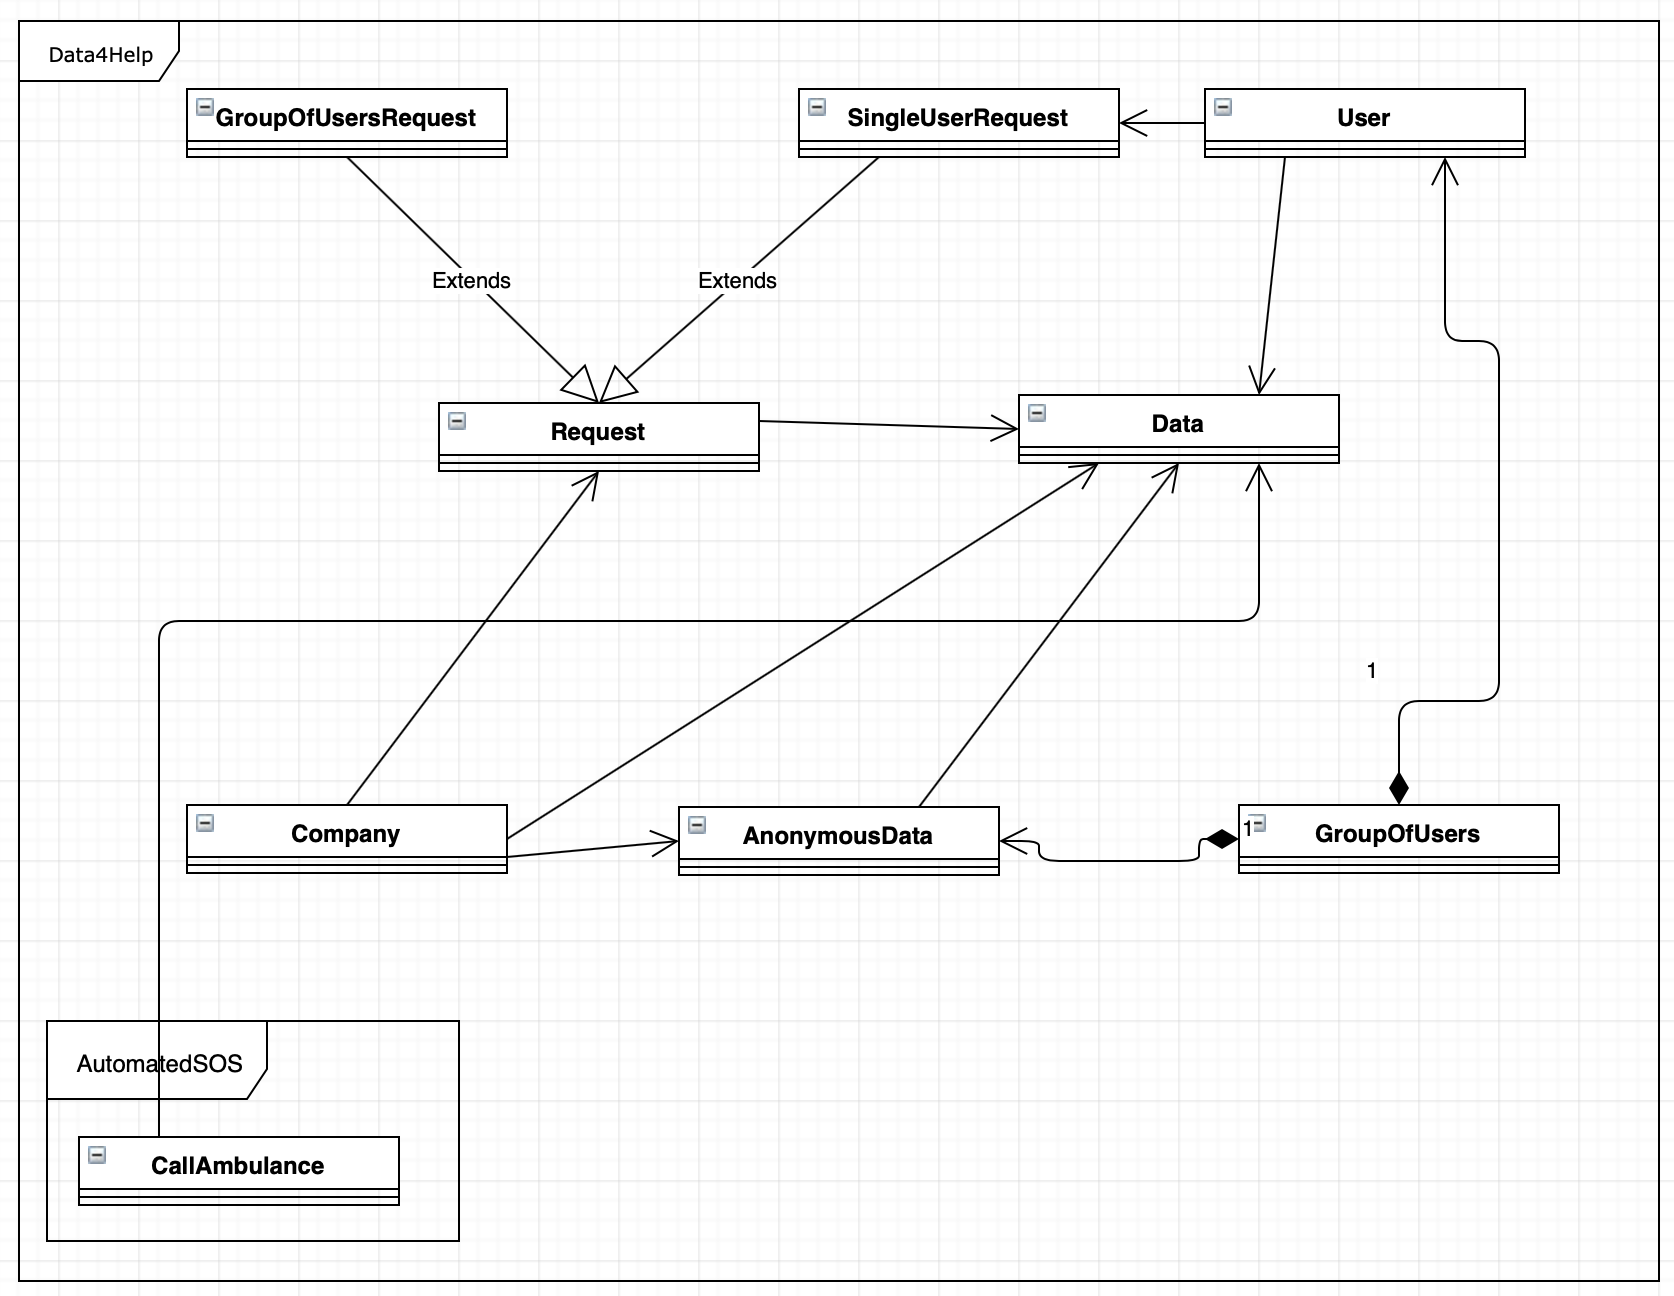
\includegraphics[width= \linewidth]{uml.png}
\end{figure}
\subsection{Product functions}
Considering all the goals previously presented, we can sum up into four categories the main functions of the product:
\subsubsection{Acquisition of users' data}
Data4Help runs on a smartwatch, assumed to be able to communicate the data directly to TrackMe's servers. It means that this product works only with smartwatch with an internet connection. Future updates will enable to use also smartwatch without internet connection to run Data4Help and AutomatedSOS.
\subsubsection{Company access to users' data}
Data4Help enables companies to access data of a specific user or of groups of users. Companies access to these data through the web page. Data are shown in a user-friendly way, generating automatically graphs. Some samples of the GUI will be shown in the corresponding section.
\subsubsection{Forwarding of following requests directly to the users and data anoymization}
Companies are able to send following requests, in order to access user data. Data4Help allows TrackMe to put in contact companies and users. Every time that a company request to access some data, Data4Help notfies TrackMe's servers. Analizing the request, TrackMe's servers will decide how to proceed:\\
\begin{itemize}
\item If the request concerns a specific user, TrackMe sends an email to the user asking to accept or reject it
\item If the request concerns a group of users, anonymizes the corresponding data 
\end{itemize}
\subsubsection{AutomatedSOS}
While registering Data4Help, the user is asked to submit his age. Basing on some creteria chosen from the managment, a value \emph{Age} is chosen. If the user's age is greater than \emph{Age} AutomatedSOS is activated automatically. AutomatedSOS is a service that monitors the heartbeat of the user and if it's lower than \emph{Threshold}, calls an ambulance addressed to the user's position within 5 seconds.
\subsection{User characteristics}
\begin{itemize}
\item \emph{Visitor}: a person not registered. The only thing he can do is proceeding with sing up.
\item \emph{User}: a person passed through a successful registration process. His data can be tracked, he can accept or reject compaines' following request.
 \item \emph{Company}: an entity that can be recognised as a company. It can see data of a specific user or anonimous data of a group of users. 
 \item \emph{TrackMe}: the whole hardware and software interfaces over which Data4Help and AutomatedSOS.
\end{itemize}
\subsection{Assumption, dependencies and constraints}
\subsubsection{Domain assumptions}
\begin{itemize}
	\item {[D1]} The user's email is already known by TrackMe.
	\item {[D2]} Only real companies can sing up as companies.
	\item {[D3]} Only companies can see users' data.
	\item {[D4]} 5 seconds are necessary to send user location and call an ambulance when parameters are below the threshold.
	\item {[D5]} Users sign up with their Google or Apple account.
	\item {[D6]} Users position is determined by using the GPS inside the smartwatch.
	\item {[D7]} When the system shows the position of a user it means that the user is
actually there.
	\item {[D8]} During the registration process the user inserts his main data (height, weight, age, place where he lives).
	\item {[D9]} The user has the physical characteristics that he inserted in the system.
	\item {[D10]} Smart watch connects directly to TrackMe and send the data acquired. Data4Help and AutomatedSOS run only on smart watch with internet access.
	\item {[D11]} The user is able to accept or reject the following requests by clicking a button on the email that TrackMe sends to him.
	\item {[D12]} Every time that a user accept or reject a following request a notification is sent to Data4Help.
	\item {[D13]} Companies have a username and a vat number and they are unique.
	\item {[D14]} Data4Help is able to anonymize data based on the group request only if the group has more than 1000 users.
	\item {[D15]} Companies know the SSN of the user. 
	\item {[D16]} A company that can see the data of a single user or of a group of users must also be able to choose the option that allows it to see users' data as soon as they are produced.
\end{itemize}\newpage
\section{Specific Requirements}
\subsection{External interface requirements}
\subsubsection{User interfaces}
\begin{figure}[h!]
\centering
    \textbf{Homepage.}\par\medskip
	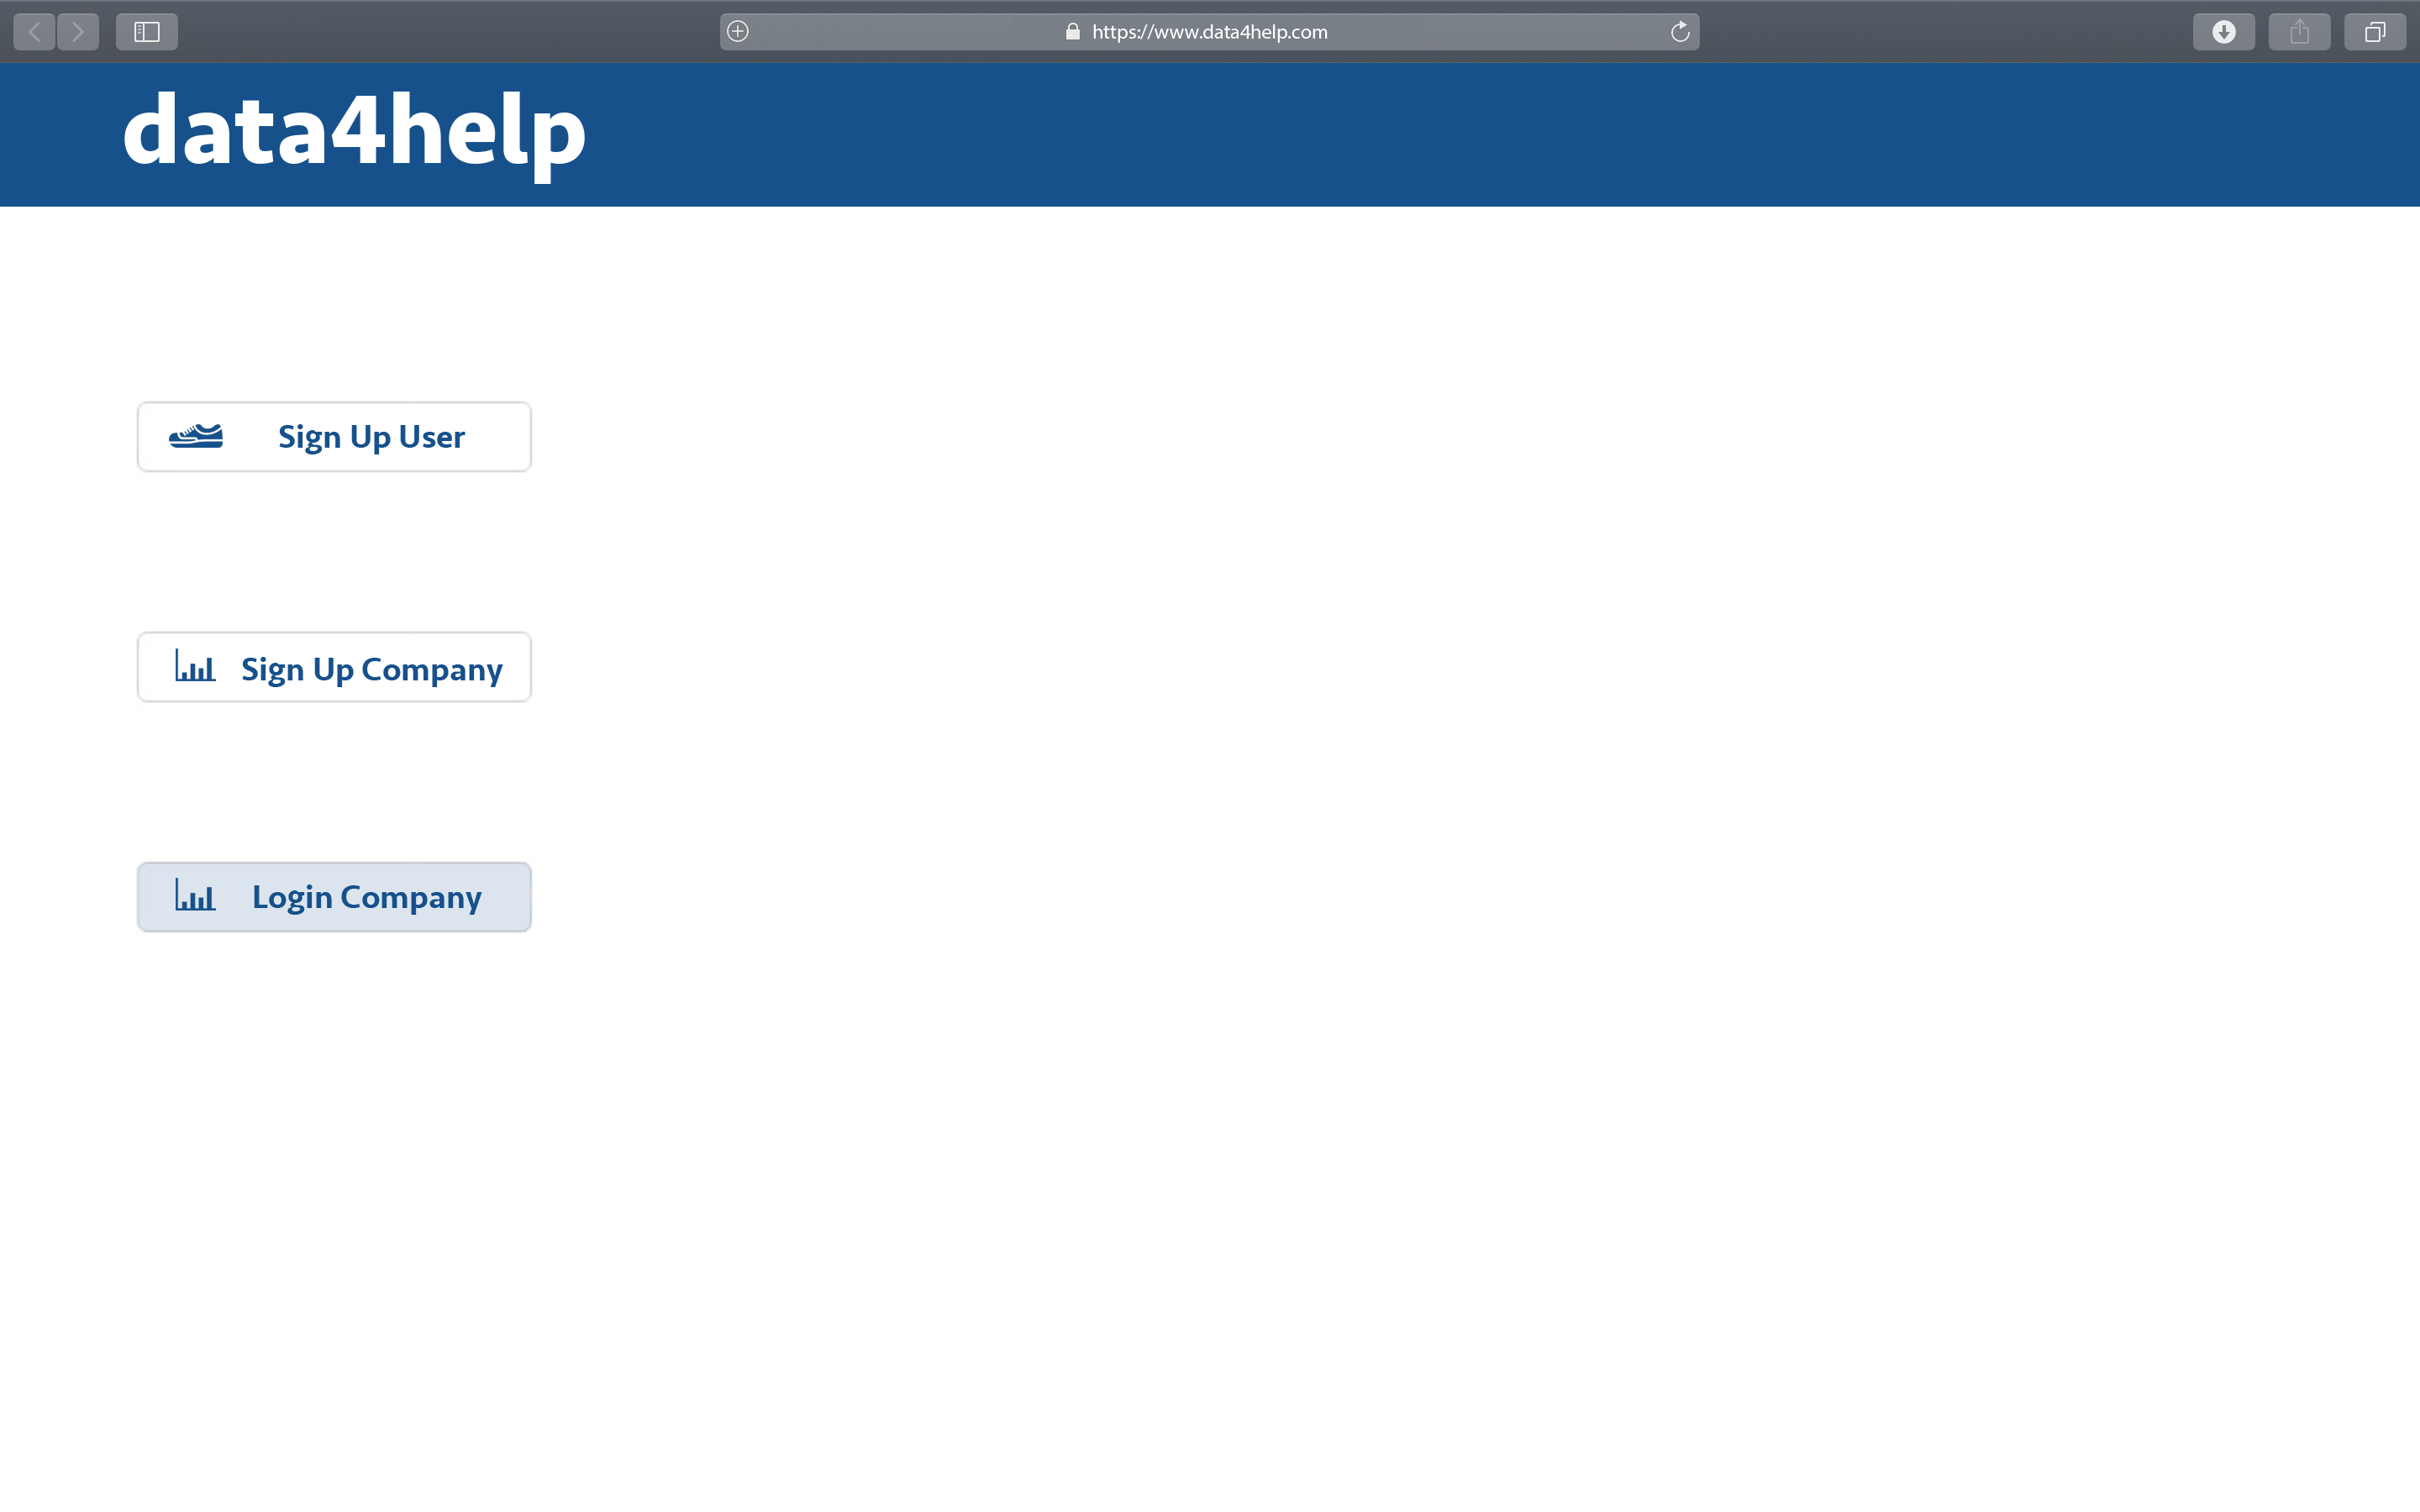
\includegraphics[width= \linewidth]{1homepage.png}
\end{figure}
\begin{figure}[h!]
\centering
    \textbf{User sign up.}\par\medskip
	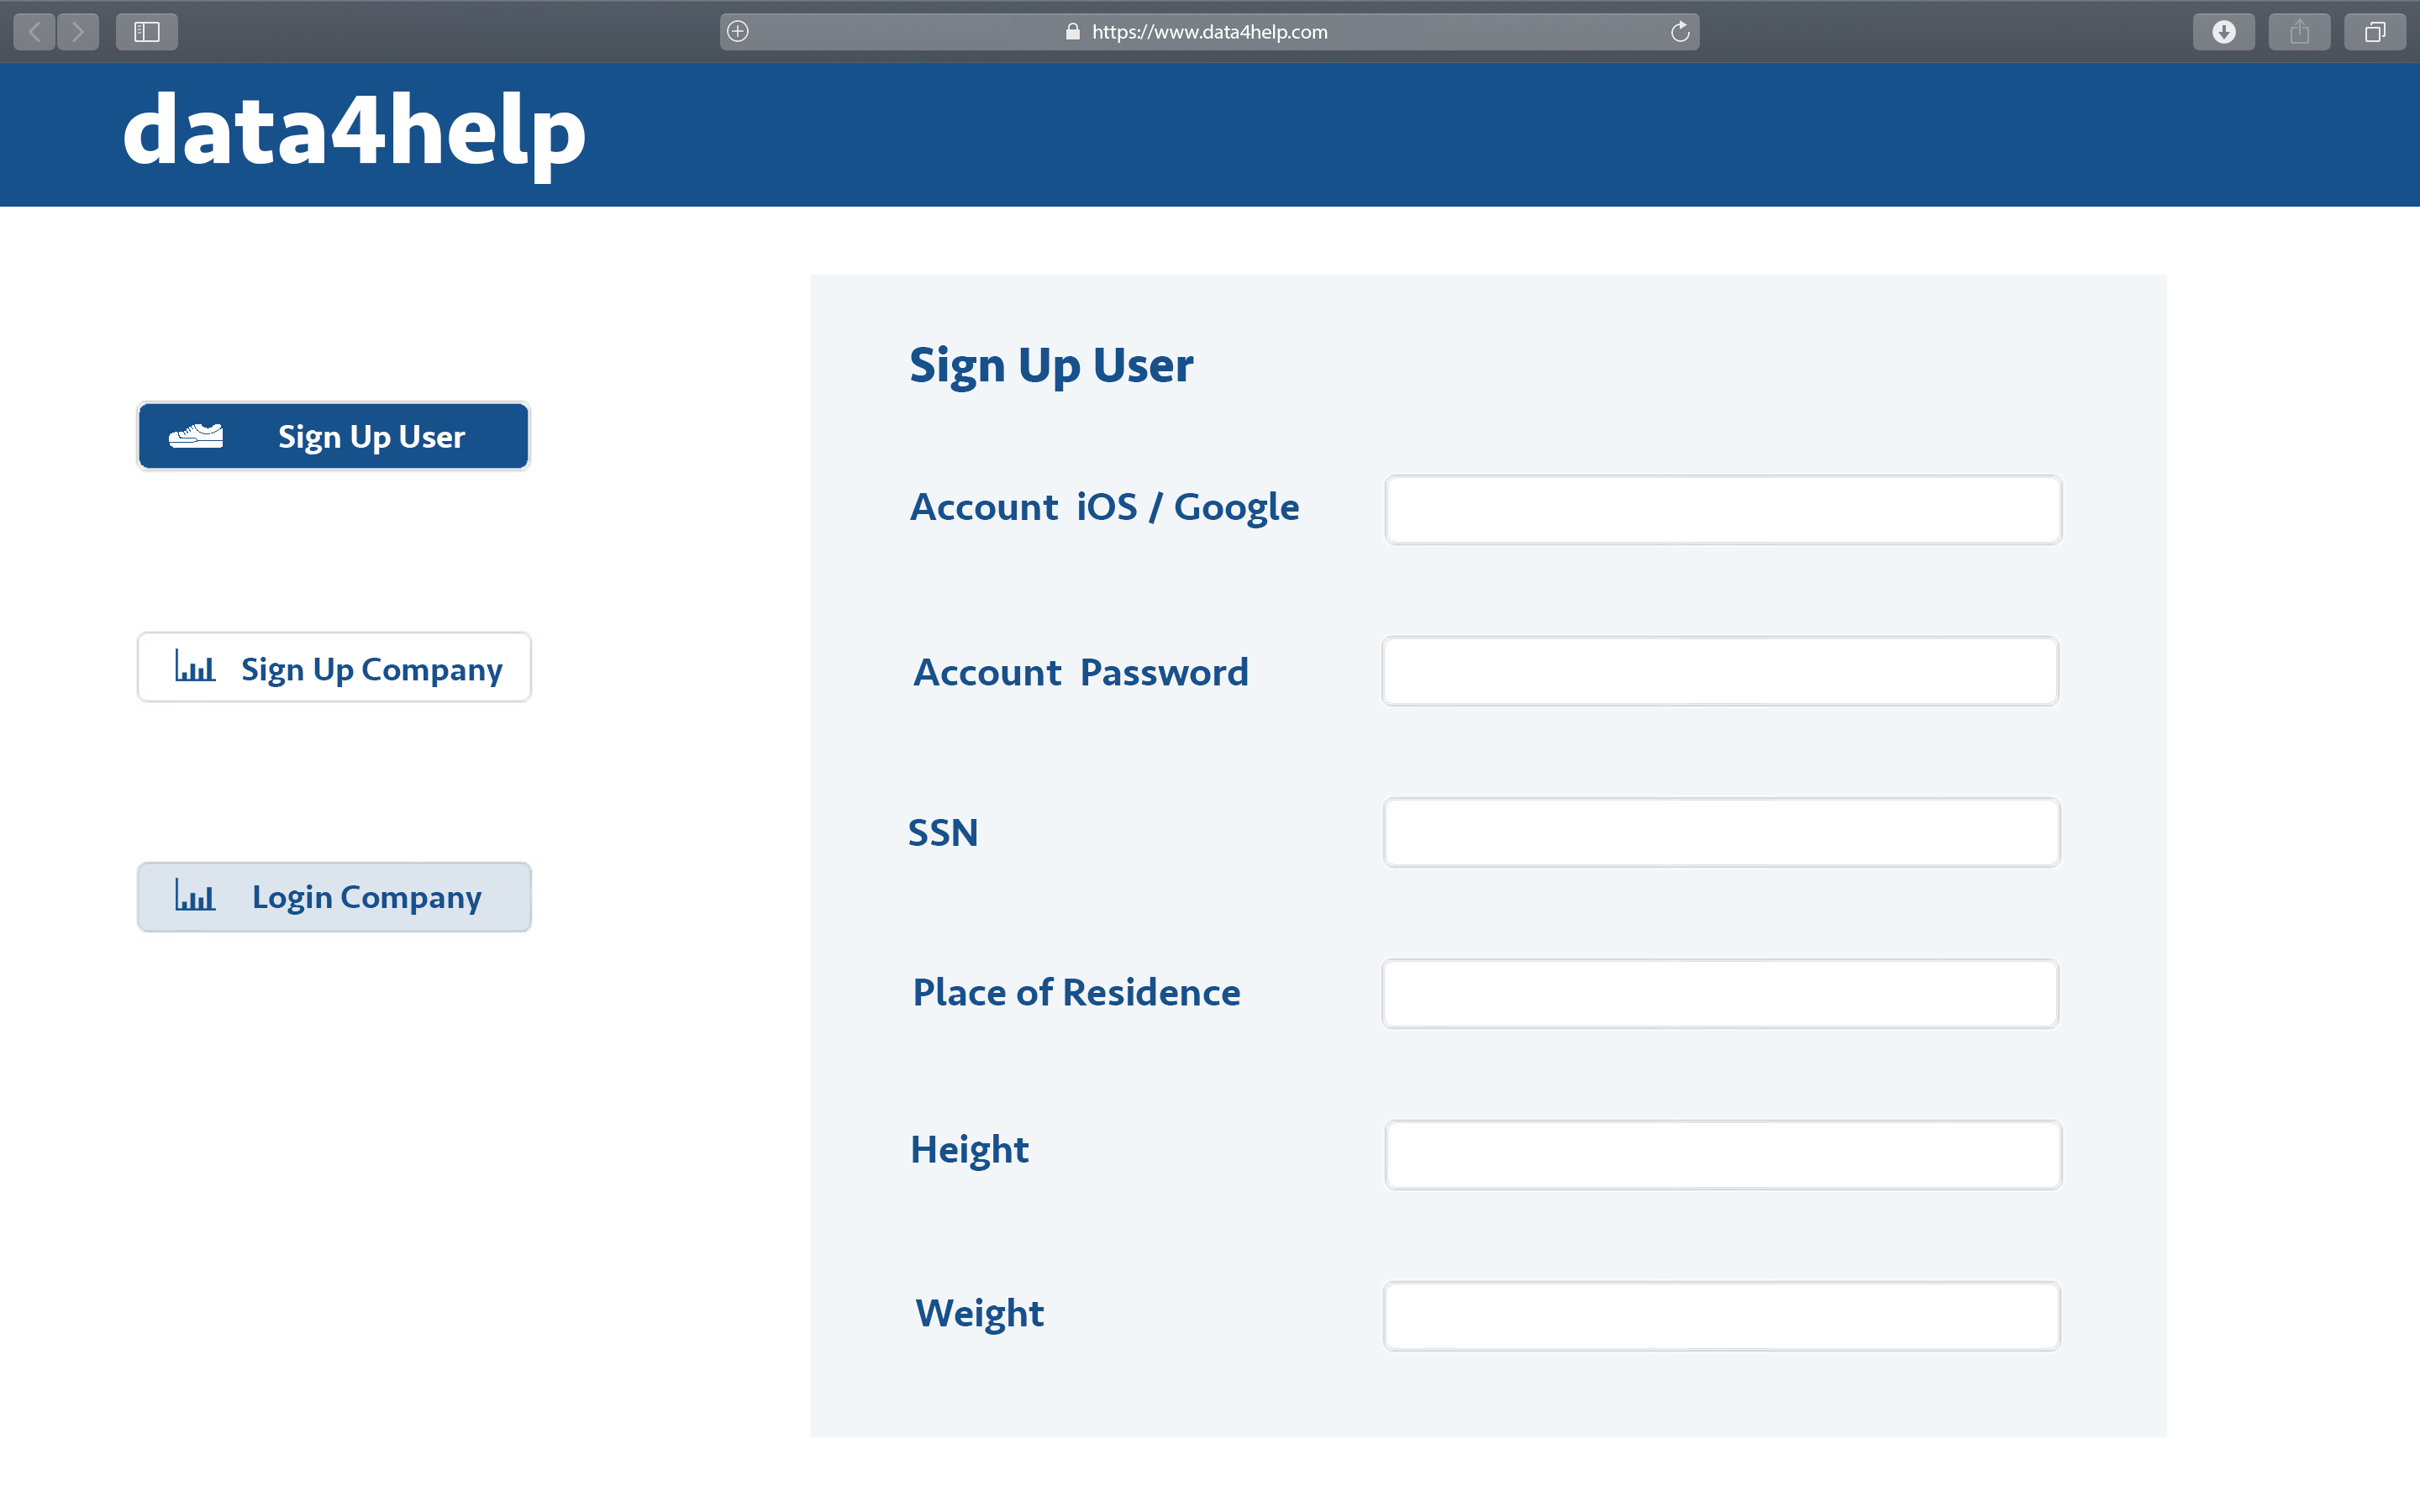
\includegraphics[width= \linewidth]{2signupuser.png}
\end{figure}\newpage
\begin{figure}[h!]
\centering
    \textbf{Company sing up.}\par\medskip
	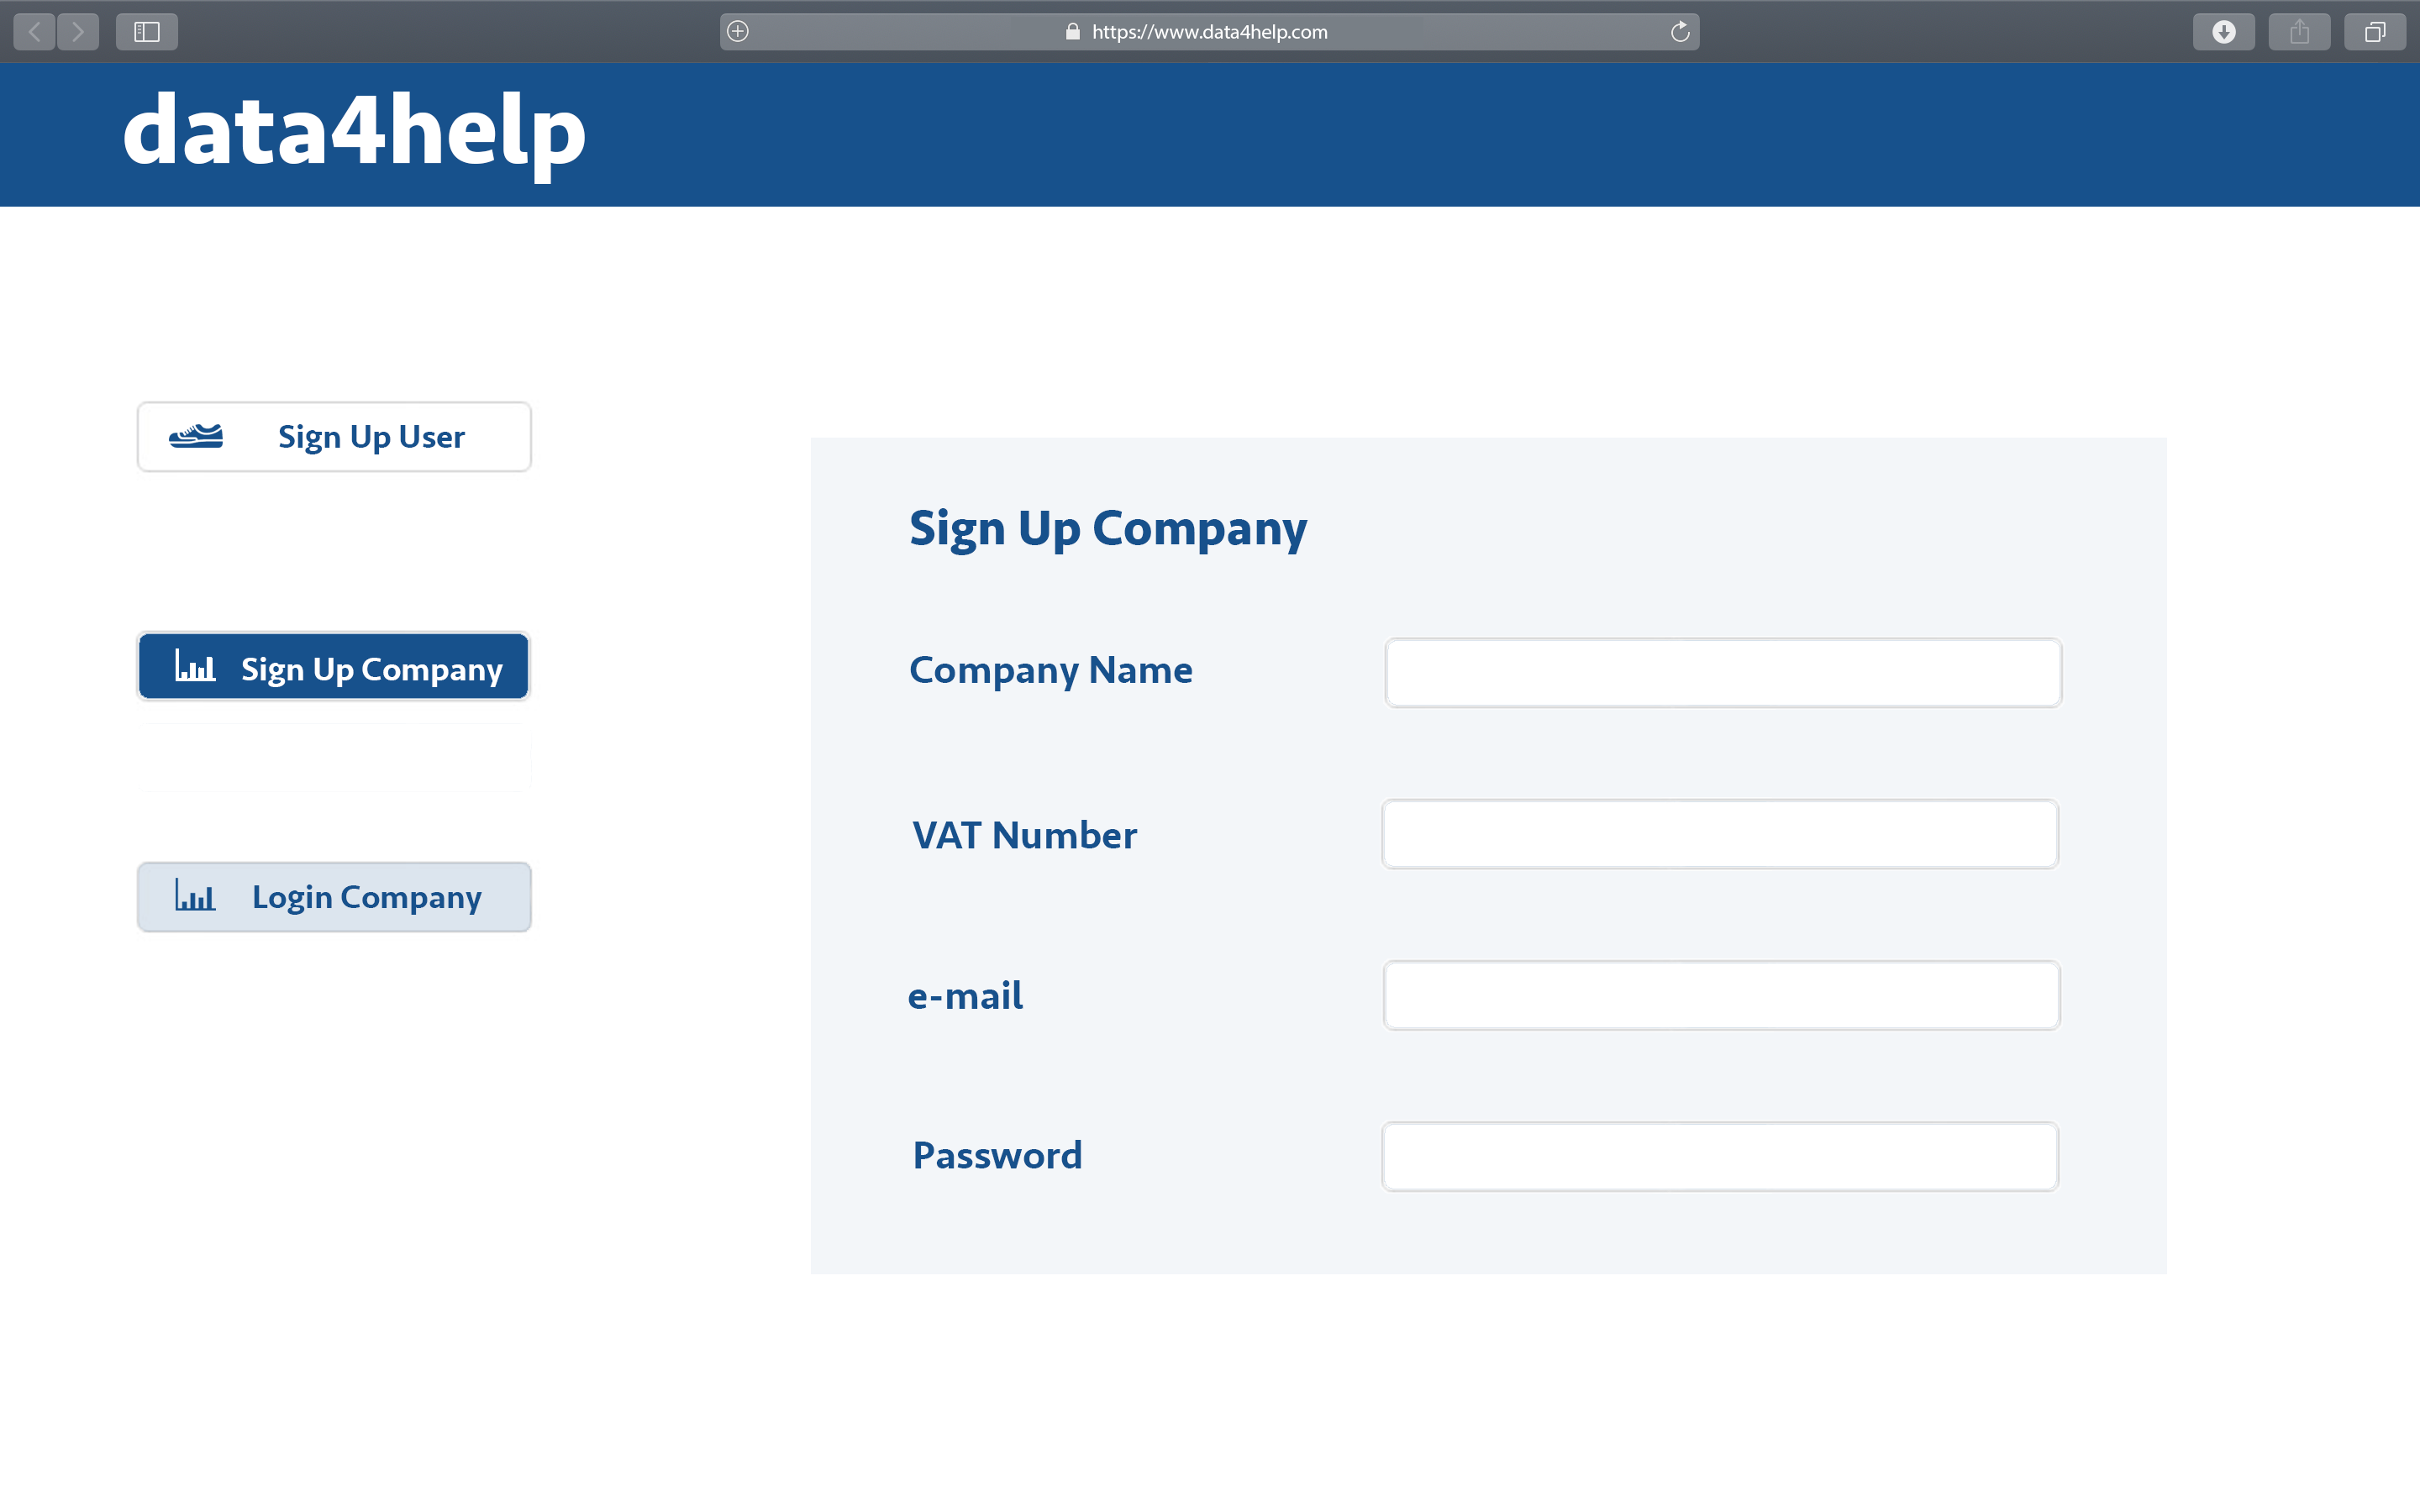
\includegraphics[width= \linewidth]{3signupcompany.png}
\end{figure}
\begin{figure}[h!]
\centering
    \textbf{Company login.}\par\medskip
	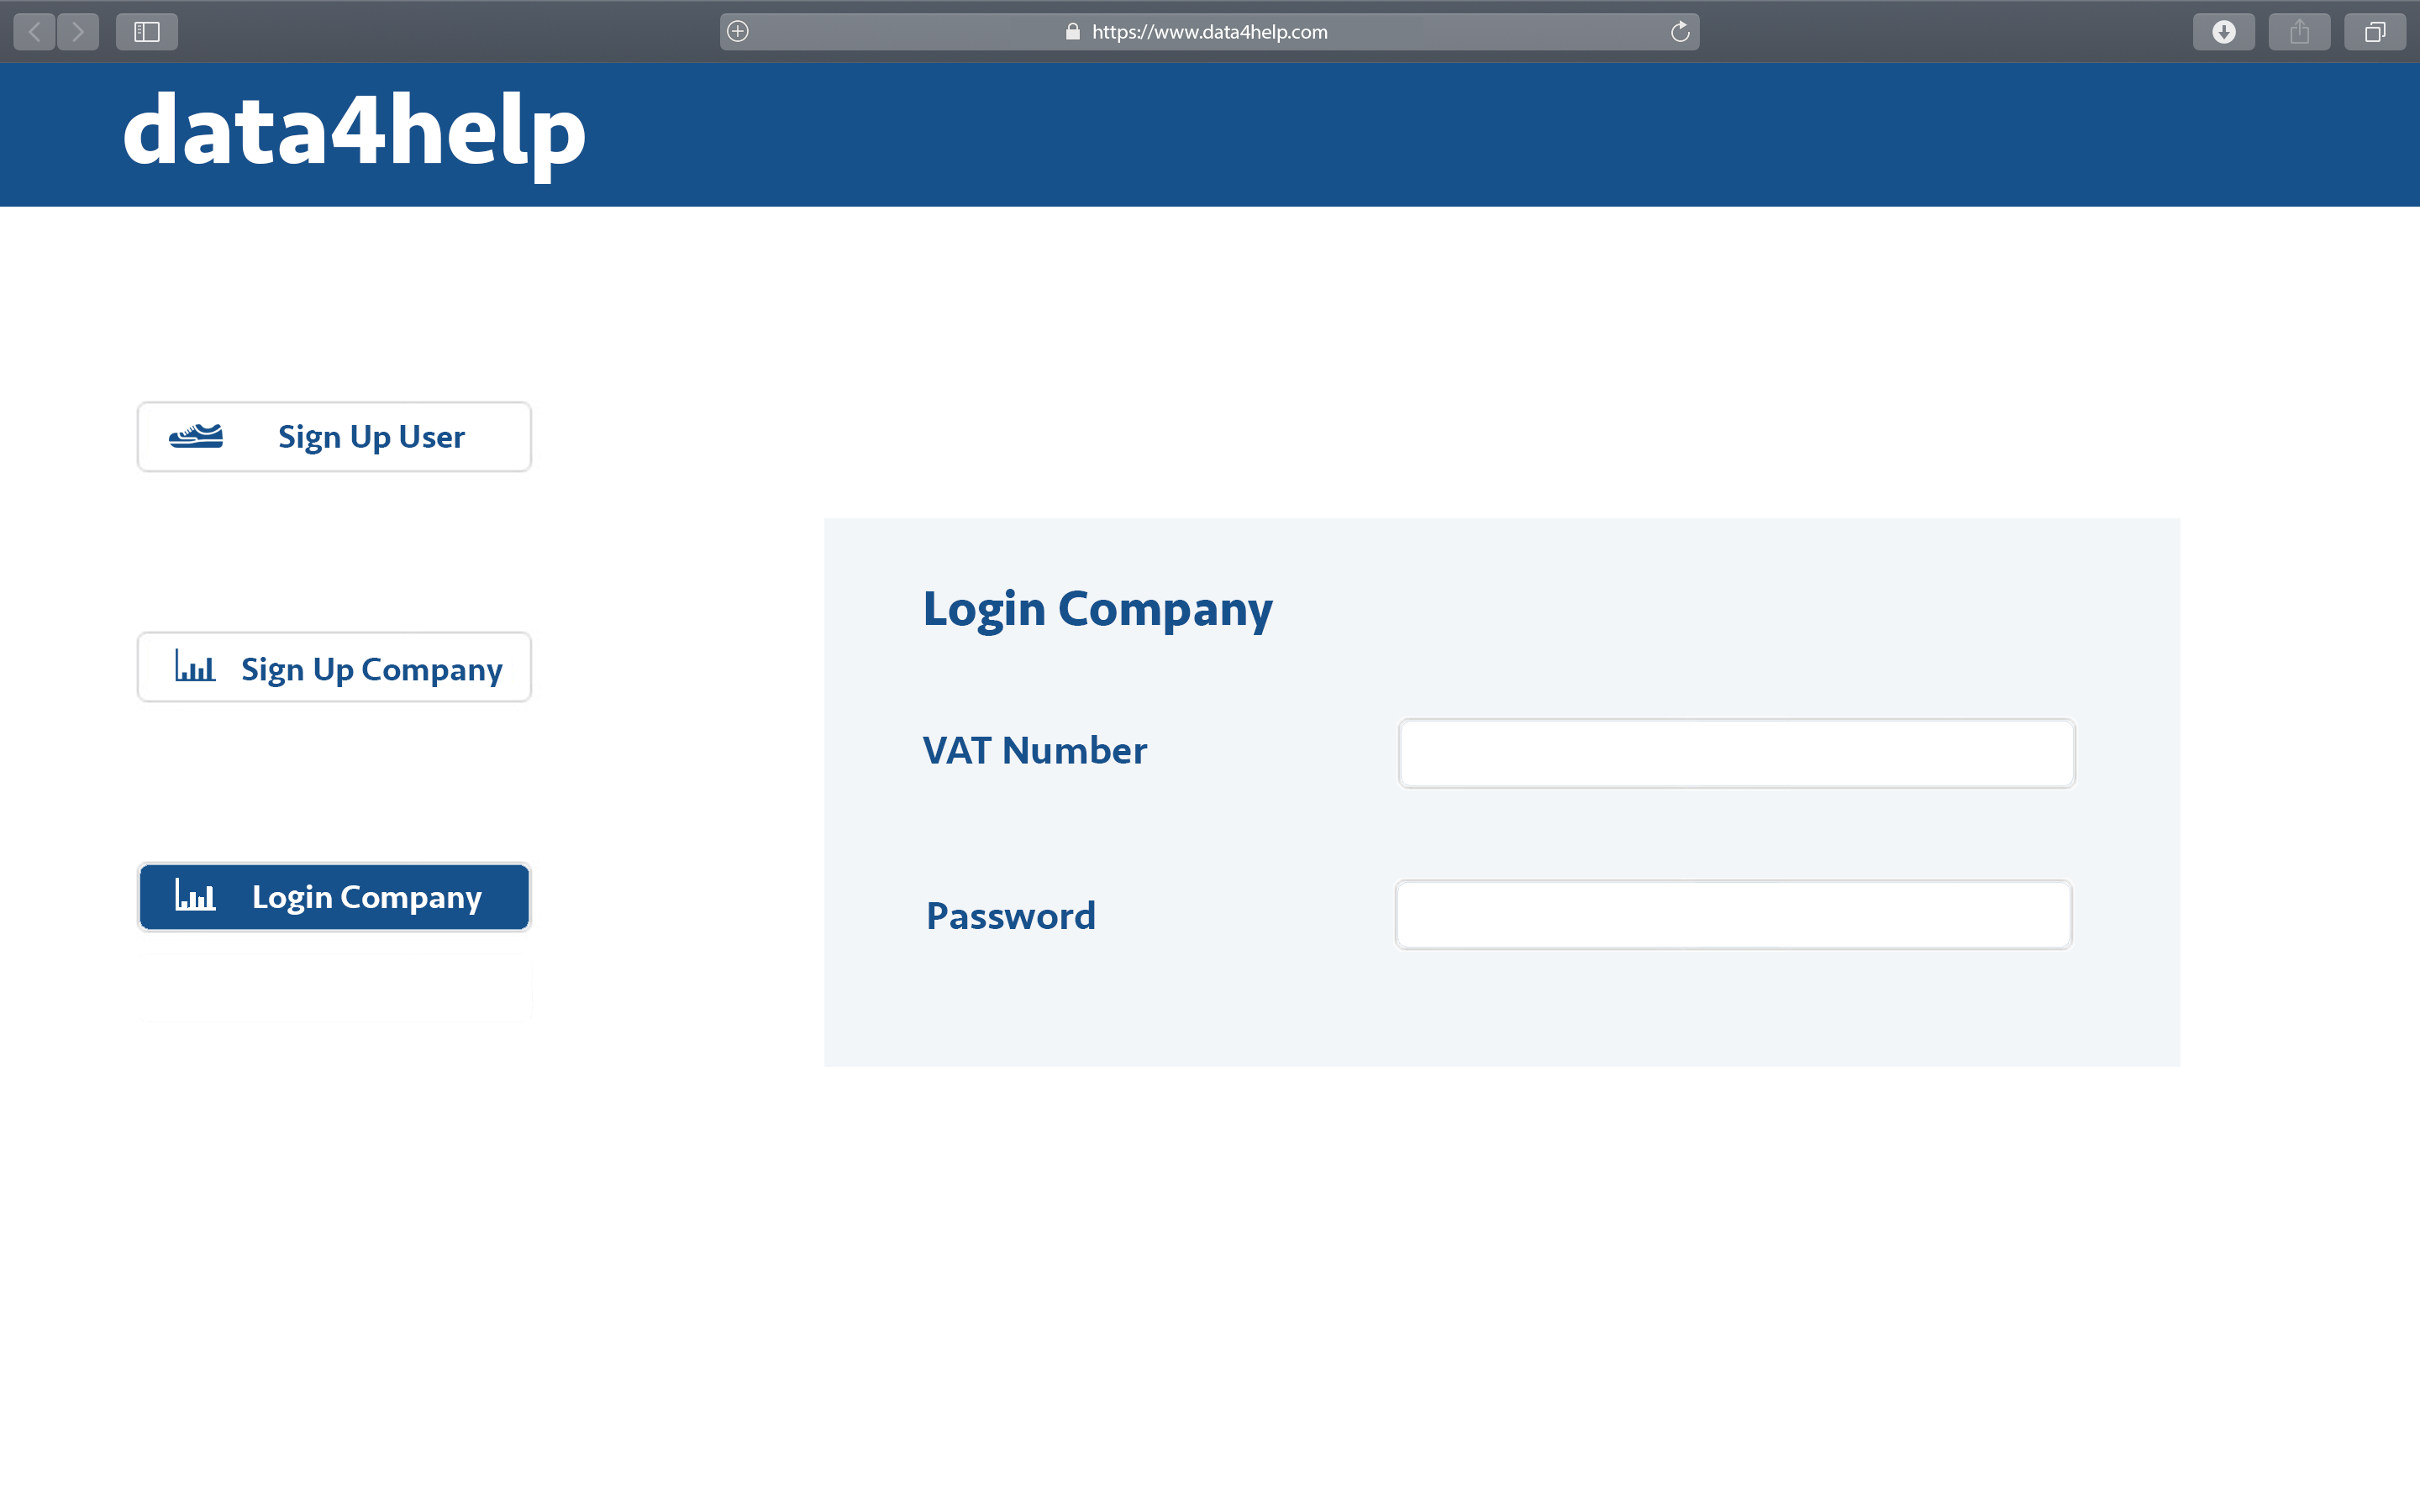
\includegraphics[width= \linewidth]{4logincompany.png}
\end{figure}\newpage
\begin{figure}[h!]
\centering
    \textbf{Requests.}\par\medskip
	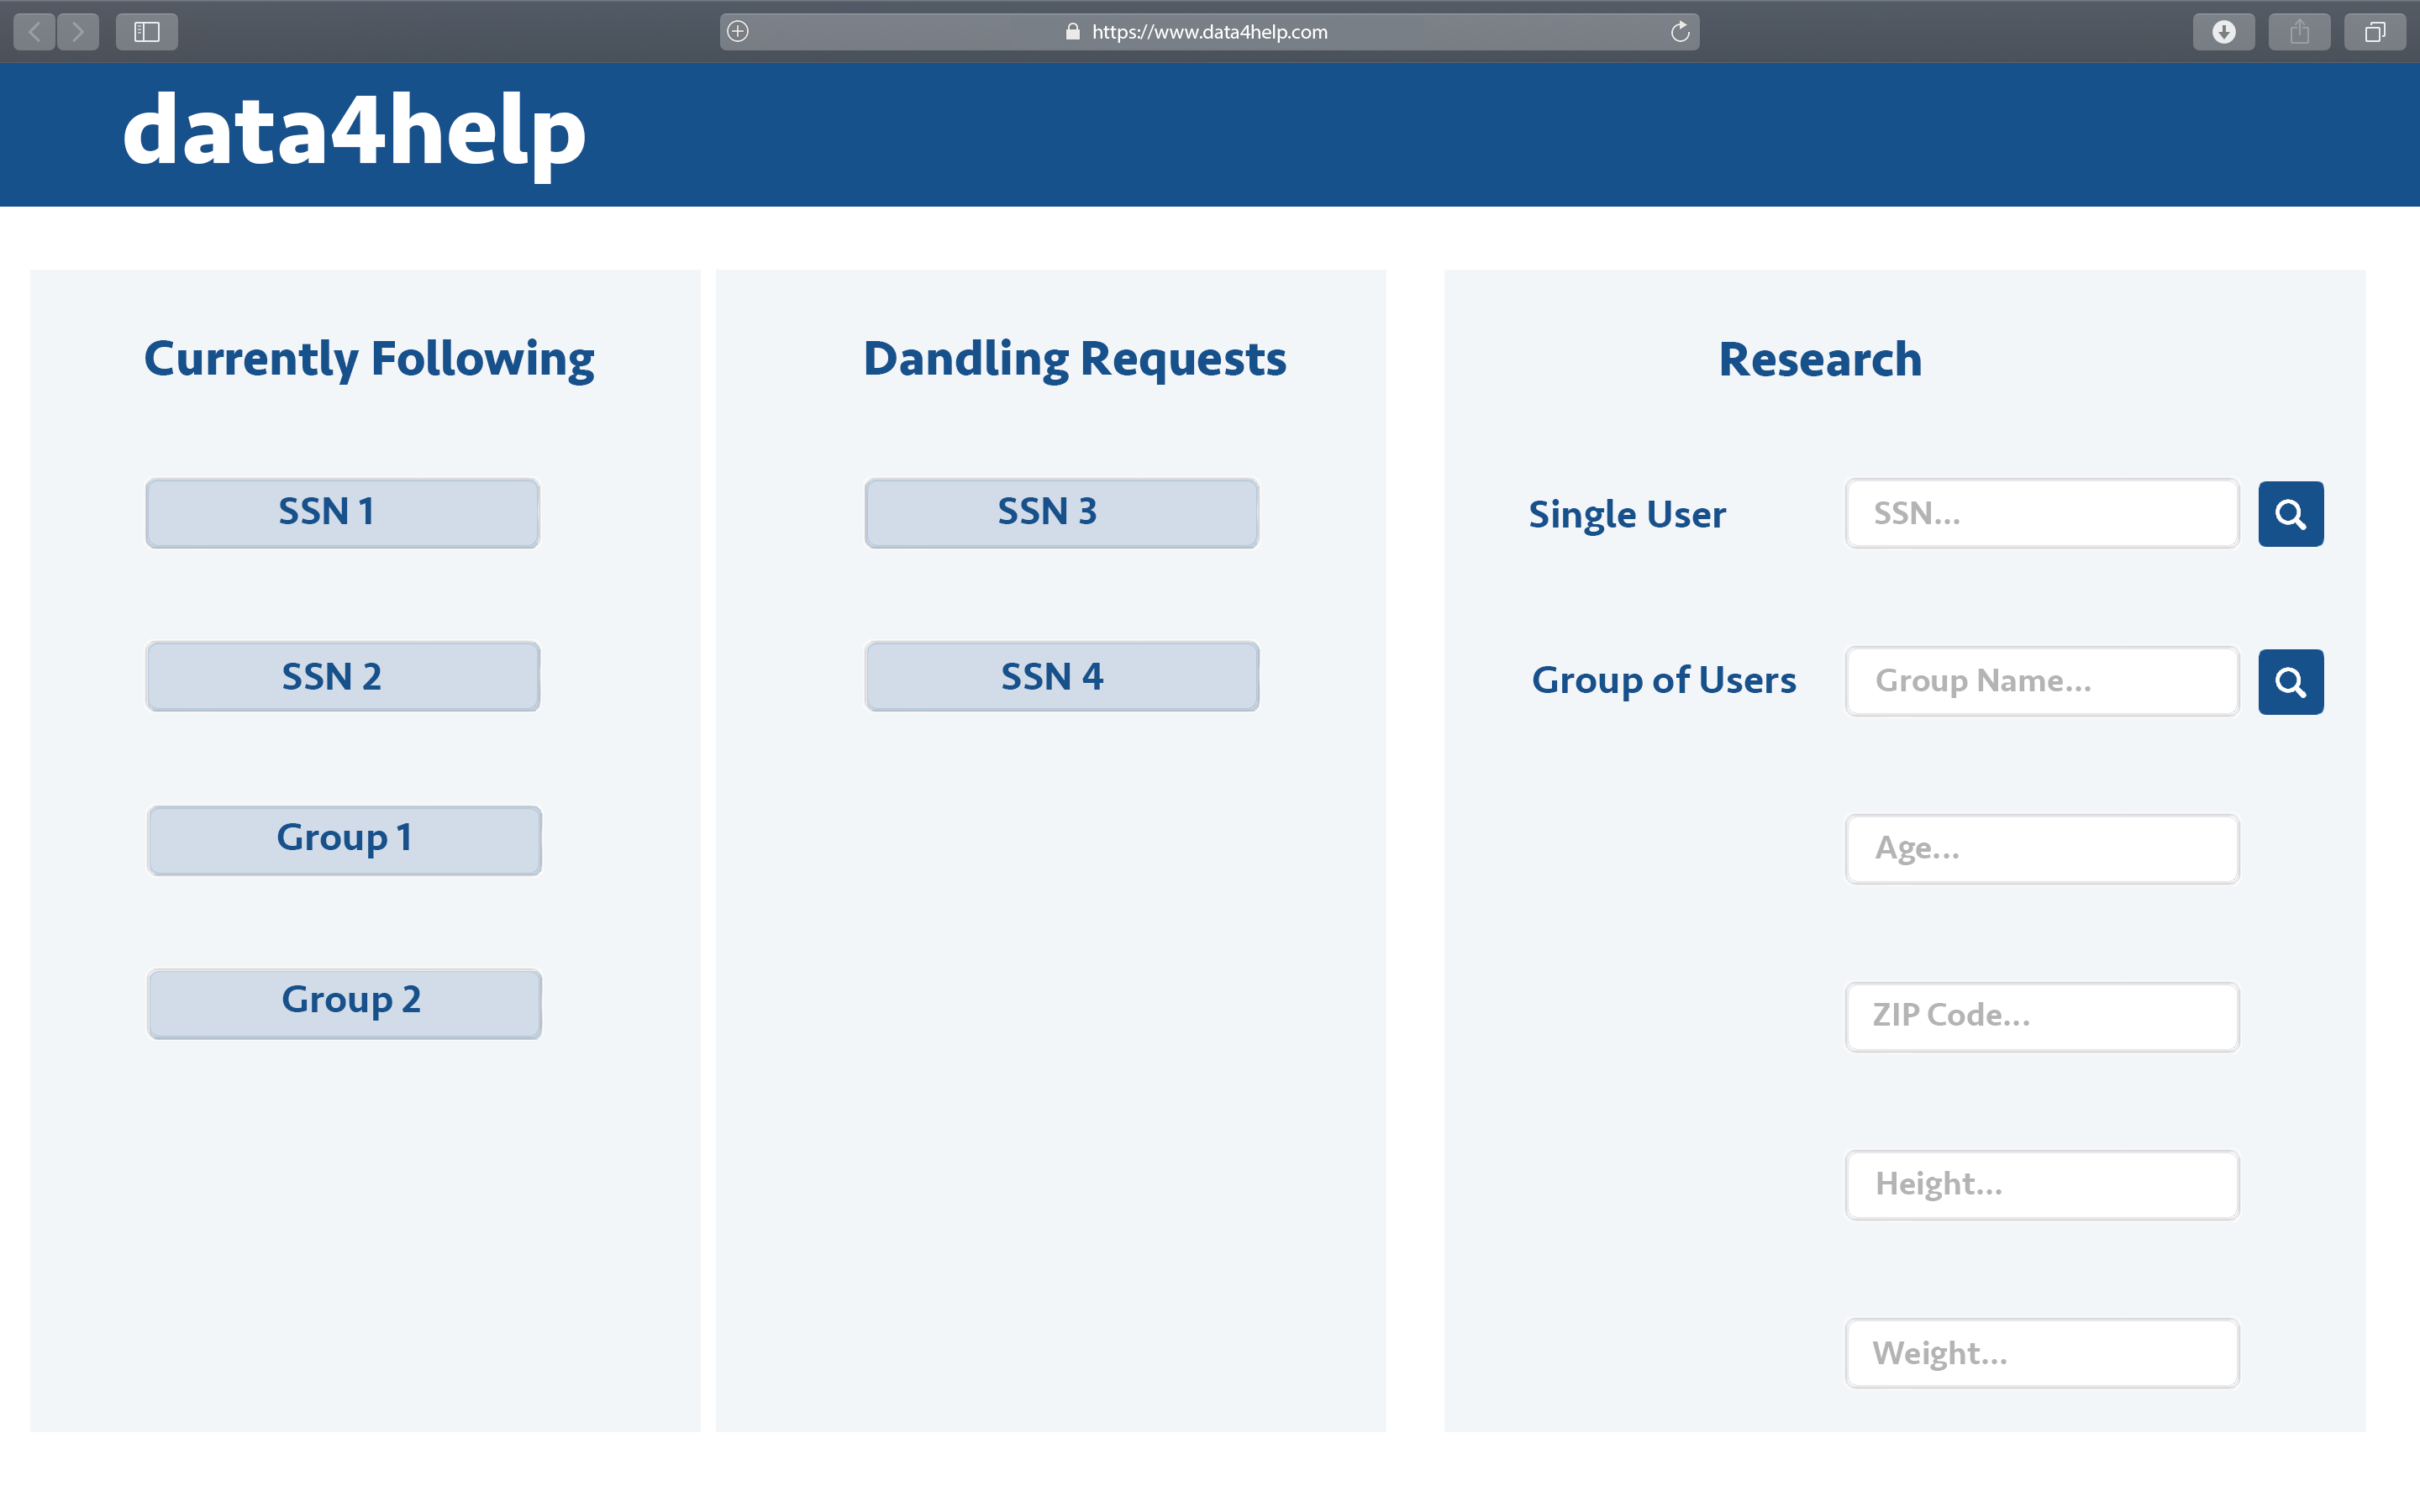
\includegraphics[width= \linewidth]{5companyhompage.png}
\end{figure}
\begin{figure}[h!]
\centering
    \textbf{Single user's data.}\par\medskip
	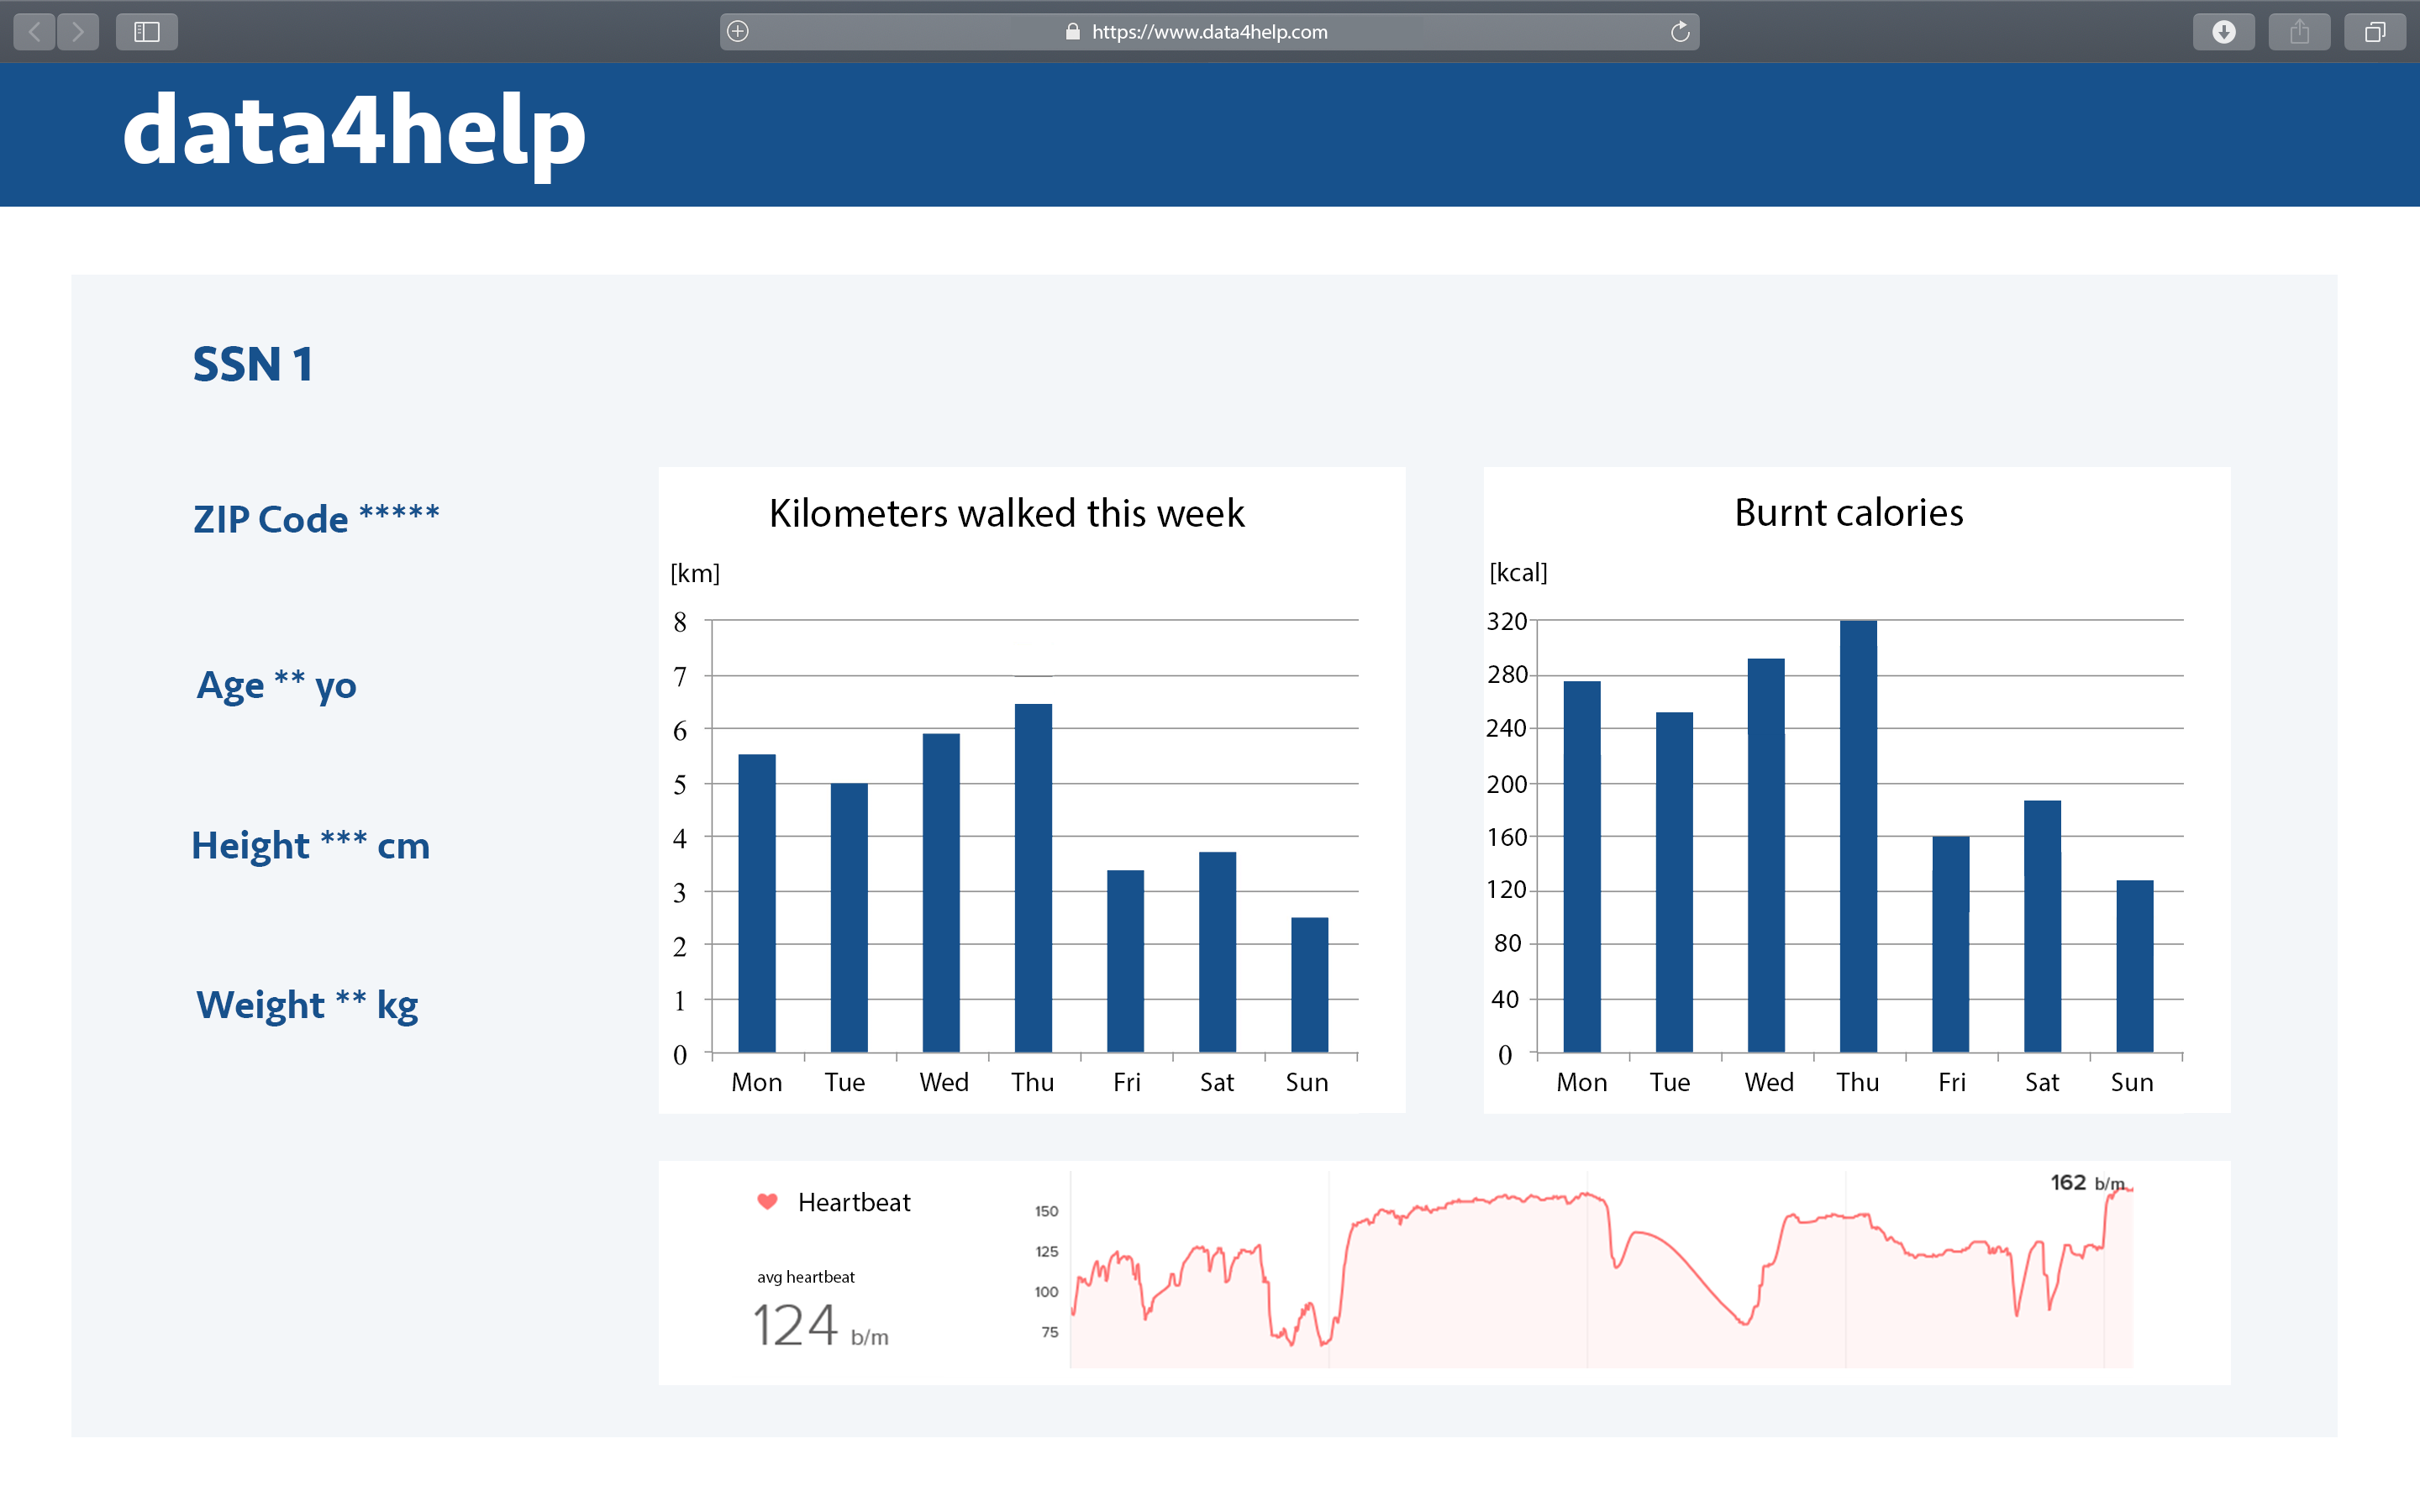
\includegraphics[width= \linewidth]{6userprofile.png}
\end{figure}\newpage
\begin{figure}[h!]
\centering
    \textbf{Group users' data.}\par\medskip
	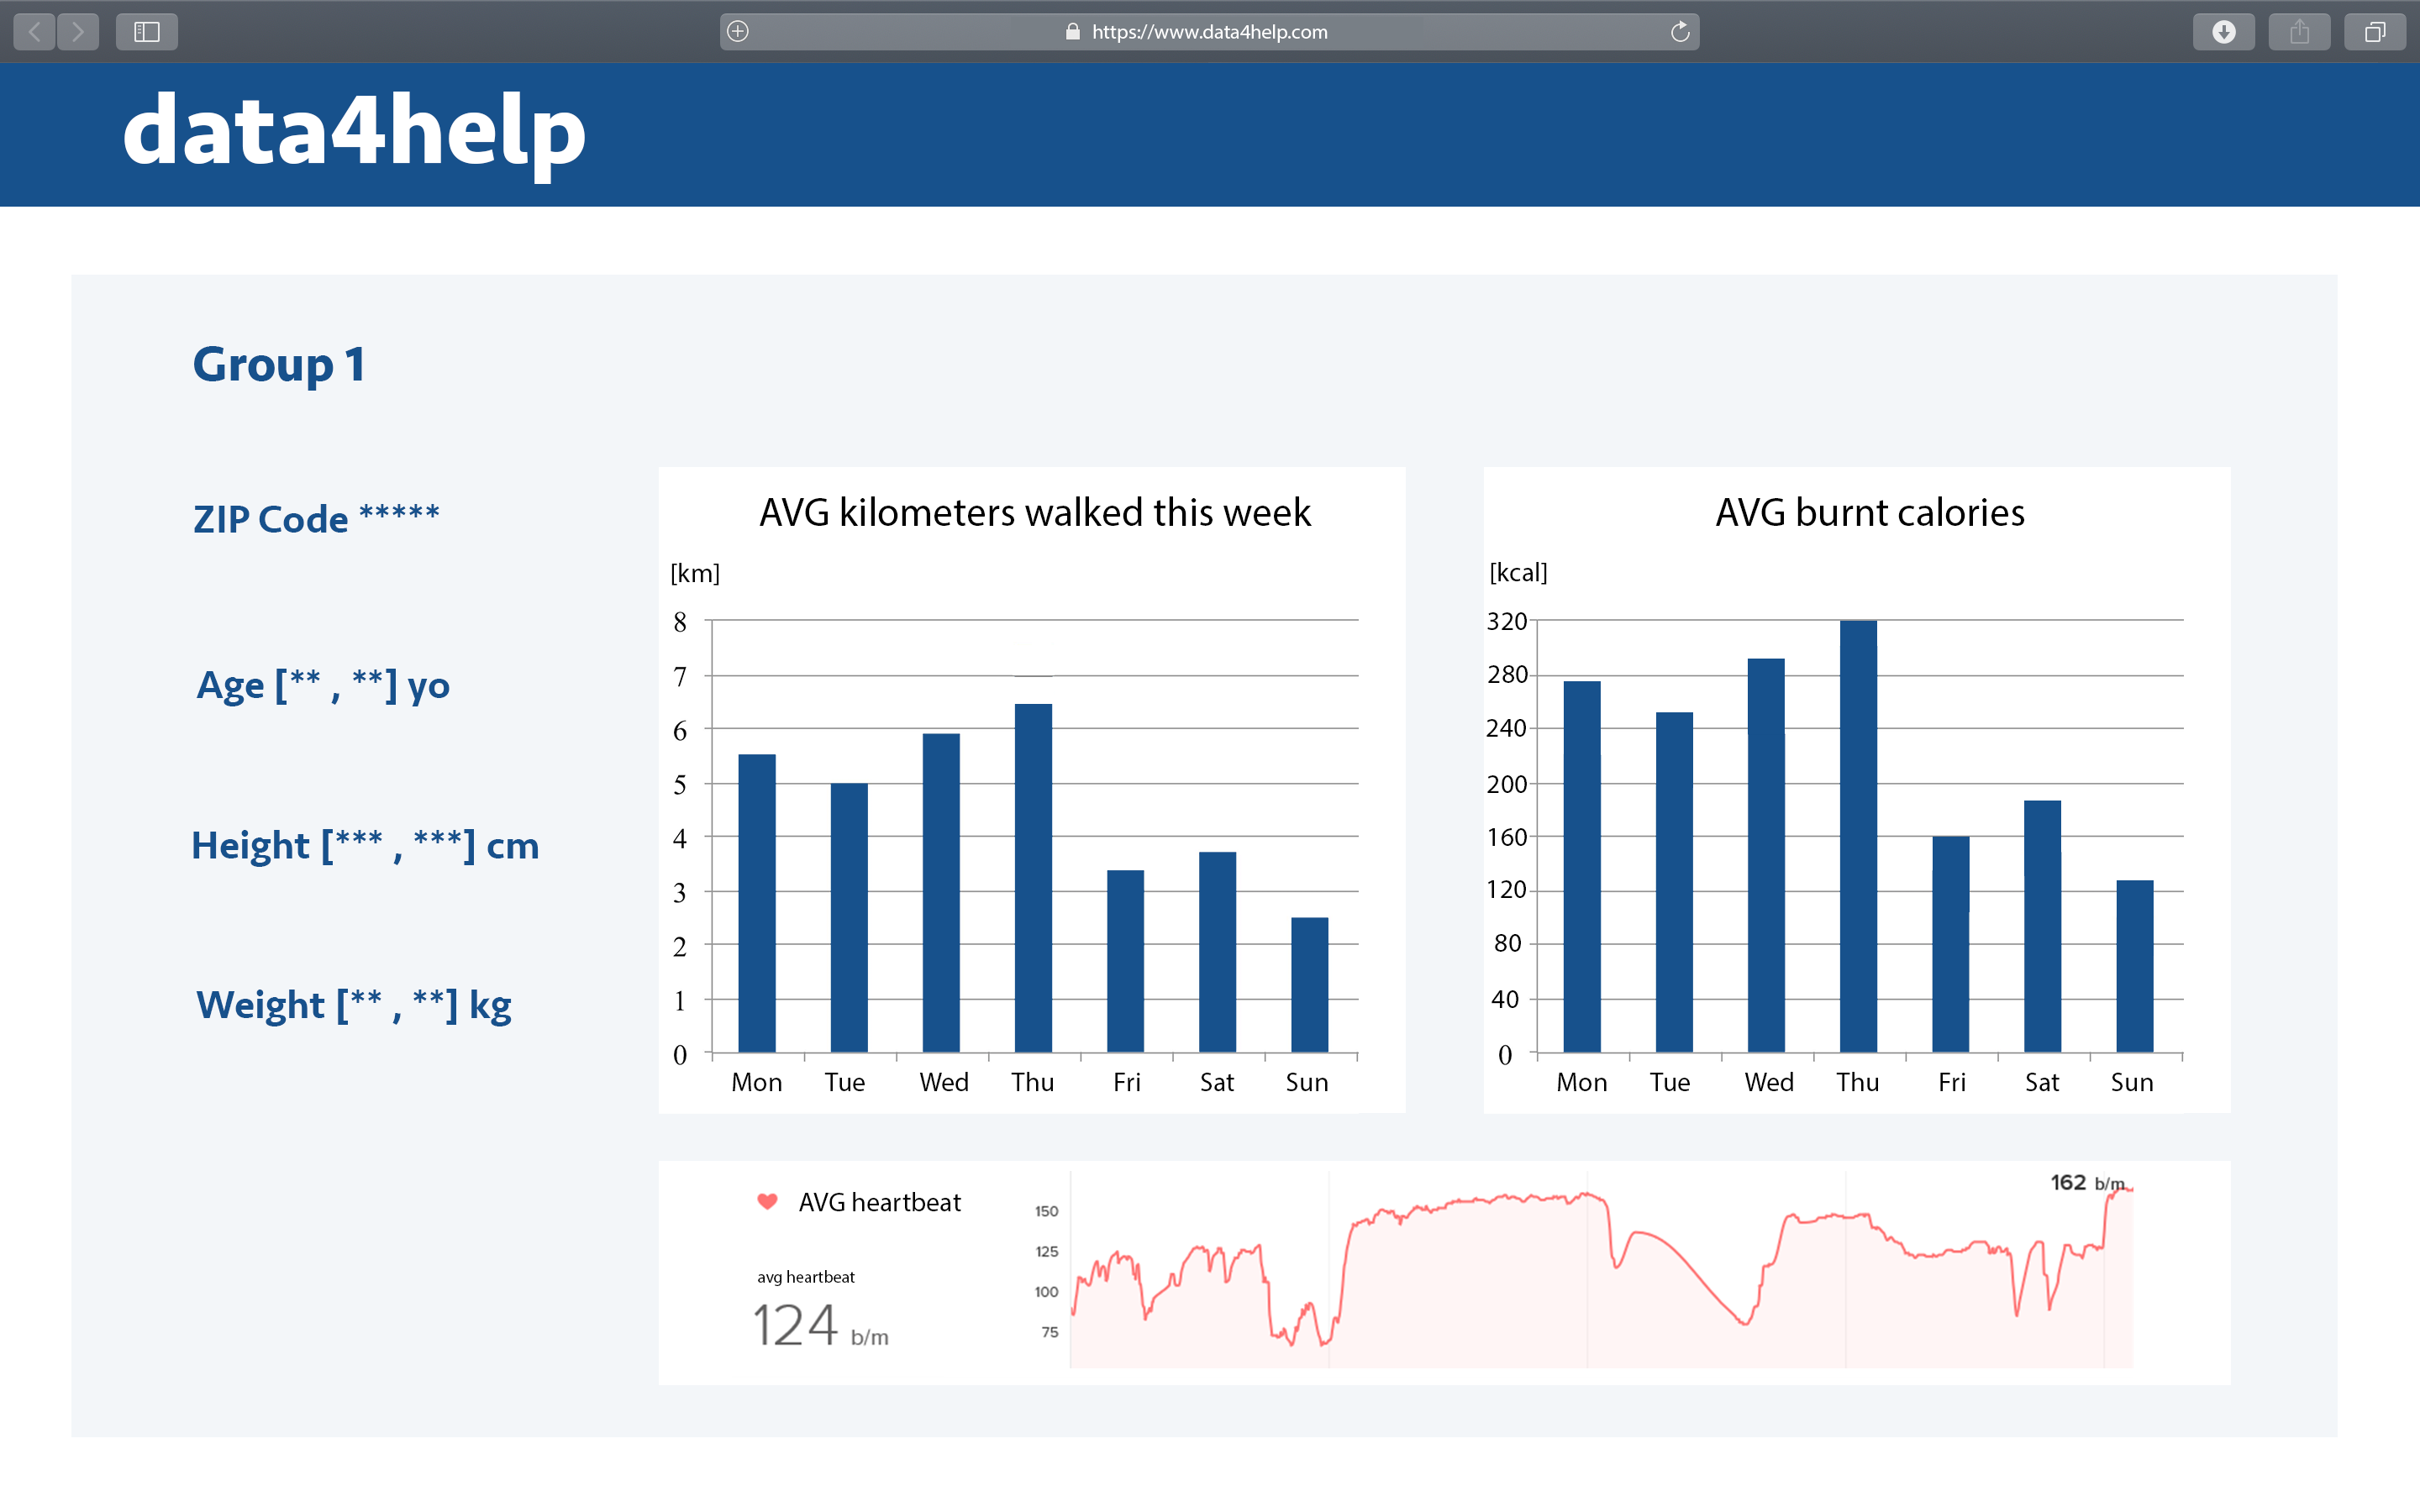
\includegraphics[width= \linewidth]{7groupprofile.png}
\end{figure}\newpage
\subsubsection{Hardware interfaces}
\begin{itemize}
	\item GPS
	\item Bluetooth
	\item Internet Connection
	\item Photoplethysmography (PPG)
	\item Accelerometer
\end{itemize}
\subsubsection{Software interfaces}
\begin{itemize}
	\item Google Maps
	\item Ambulance Service
\end{itemize}
\subsubsection{Communication interfaces}
This network-connected background app uses LTE to send and receive data.
\subsection{Scenarios}
\subsection{Functional requirements}
\subsubsection{[G1] Visitor can become User after providing credentials.}
\begin{itemize}
\item {[R1]} The system must allow a visitor to begin the registration process. During the process the system will ask him to provide credentials.
\item {[D5]} Users sign up with their Google or Apple account.
\item {[D8]} During the registration process the user inserts his main data (height, weight, age, place where he lives).
\item {[D9]} The user has the physical characteristics that he inserted in the system.
\end{itemize}
\subsubsection{[G2] User can accept or reject the request of access to his data formulated by companies.}
\begin{itemize}
\item {[D1]} The user's email is already known by TrackMe.
\item {[D11]} The user is able to accept or reject the following requests by clicking a button on the email that TrackMe sends to him.
\item {[D12]} Every time that a user accept or reject a following request a notification is sent to Data4Help.
\item {[R2]} Each time that an accepting or rejecting notification is sent to Data4Help, the system must mark a \emph{Pendent User} as not pendent anymore.
\item {[R3]} Each time that a user changes state from pendent to non-pendent, the corresponding single user request in the company list moves from dandling to accepted.
\end{itemize}
\subsubsection{[G3] If user's parameters are below specified thresholds, an ambulance is called within 5 seconds. [G3.1] Ambulance is required at current user's location.}
\begin{itemize}
\item {[R4]} The system must be able to monitor the user heart rate through hardware interfaces that are installed in the smart watch.
\item {[D10]} Smart watch connects directly to TrackMe and send the data acquired. Data4Help and AutomatedSOS run only on smart watch with internet access.
\item {[D6]} Users position is determined by using the GPS inside the smartwatch.
\item {[D7]} When the system shows the position of a user it means that the user is actually there.
\item {[D4]} 5 seconds are necessary to send user location and call an ambulance when parameters are below the threshold.
\end{itemize}
\subsubsection{[G4] Company can sign up as Company to Data4Help and AutomatedSOS.}
\begin{itemize}
\item {[R5]} The system must allow a company to begin the registration process. During the process the system will ask to provide credentials.
\item {[D2]} Only real companies can sing up as compaines.
\item {[R6]} At the end of the registration process, the system must provide to the company a username and a password.
\item {[D13]} Companies have a username and a vat number and they are unique.
\end{itemize}
\subsubsection{[G5] Company can be recognized providing a password and vat number.}
\begin{itemize}
\item {[D13]} Companies have a username and a vat number and they are unique.
\item {[R7]} The company can log in to the website by providing the combination of a username and a password that match its account.
\end{itemize}
\subsubsection{[G6] Company can formulate a request to see anonymized data of a group of users.}
\begin{itemize}
\item {[R8]} The system must allow the company to formulate a group of users request.
\item {[R9]} The system must allow the company to fill in the request via a drop down menu.
\item {[R10]} The system must allow the company to send a notification to TrackMe software interfaces.
\end{itemize}
\subsubsection{[G7] Company can formulate a request to see data of a specific user providing his SSN.}
\begin{itemize}
\item {[R11]} The system must allow the company to formulate a single user request.
\item {[R12]} The system must allow the company to fill in the request by inserting the user's SSN.
\item {[R10]} The system must allow the company to send a notification to TrackMe software interfaces.
\end{itemize}
\subsubsection{[G8] Company can see anonymized data of a group of users.}
\begin{itemize}
\item {[D3]} Only companies can see users’ data.
\item {[D14]} TrackMe is able to anonymize data based on the group request only if the group has more than 1000 users.
\item {[R13]} The system must allow companies to see the data that TrackMe was able to anonymize and for which exist the group request.
\end{itemize}
\subsubsection{[G9] Company can see data of a specific user providing his SSN.}
\begin{itemize}
\item {[D3]} Only companies can see users’ data.
\item {[D15]} Companies know the SSN of the user.
\item {[D16]} The system must allow companies to see data of a single user if the single user request exists and if the user approved that request.
\end{itemize}
\subsubsection{[G10] Company can subscribe to users’ new data.}
\begin{itemize}
\item {[D3]} Only companies can see users’ data.
\item {[R14]} The system must allow companies to see users' data as soon as they are produced.
\item {[D16]} A company that can see the data of a single user or of a group of users must also be able to choose the option that allows it to see users' data as soon as they are produced.
\end{itemize}
\subsubsection{[G11] Data4Help can anonymise data.}
\begin{itemize}
\item {[D14]} Data4Help is able to anonymize data based on the group request only if the group has more than 1000 users.
\item {[R15]} The system must be able to anonymize data.
\end{itemize}
\subsubsection{[G12] Data4Help can forward companies’ requests to users.}
\begin{itemize}
\item {[D1]} The user’s email is already known by TrackMe.
\item {[R10]} The system must allow the company to send a notification to TrackMe software interfaces.
\item {[R16]} The system must allow TrackMe to send an email to the user in order to enable the company to see his data.
\end{itemize}\newpage
\subsubsection{Use case diagram}

\begin{figure}[h!]
\centering
    \textbf{}\par\medskip
	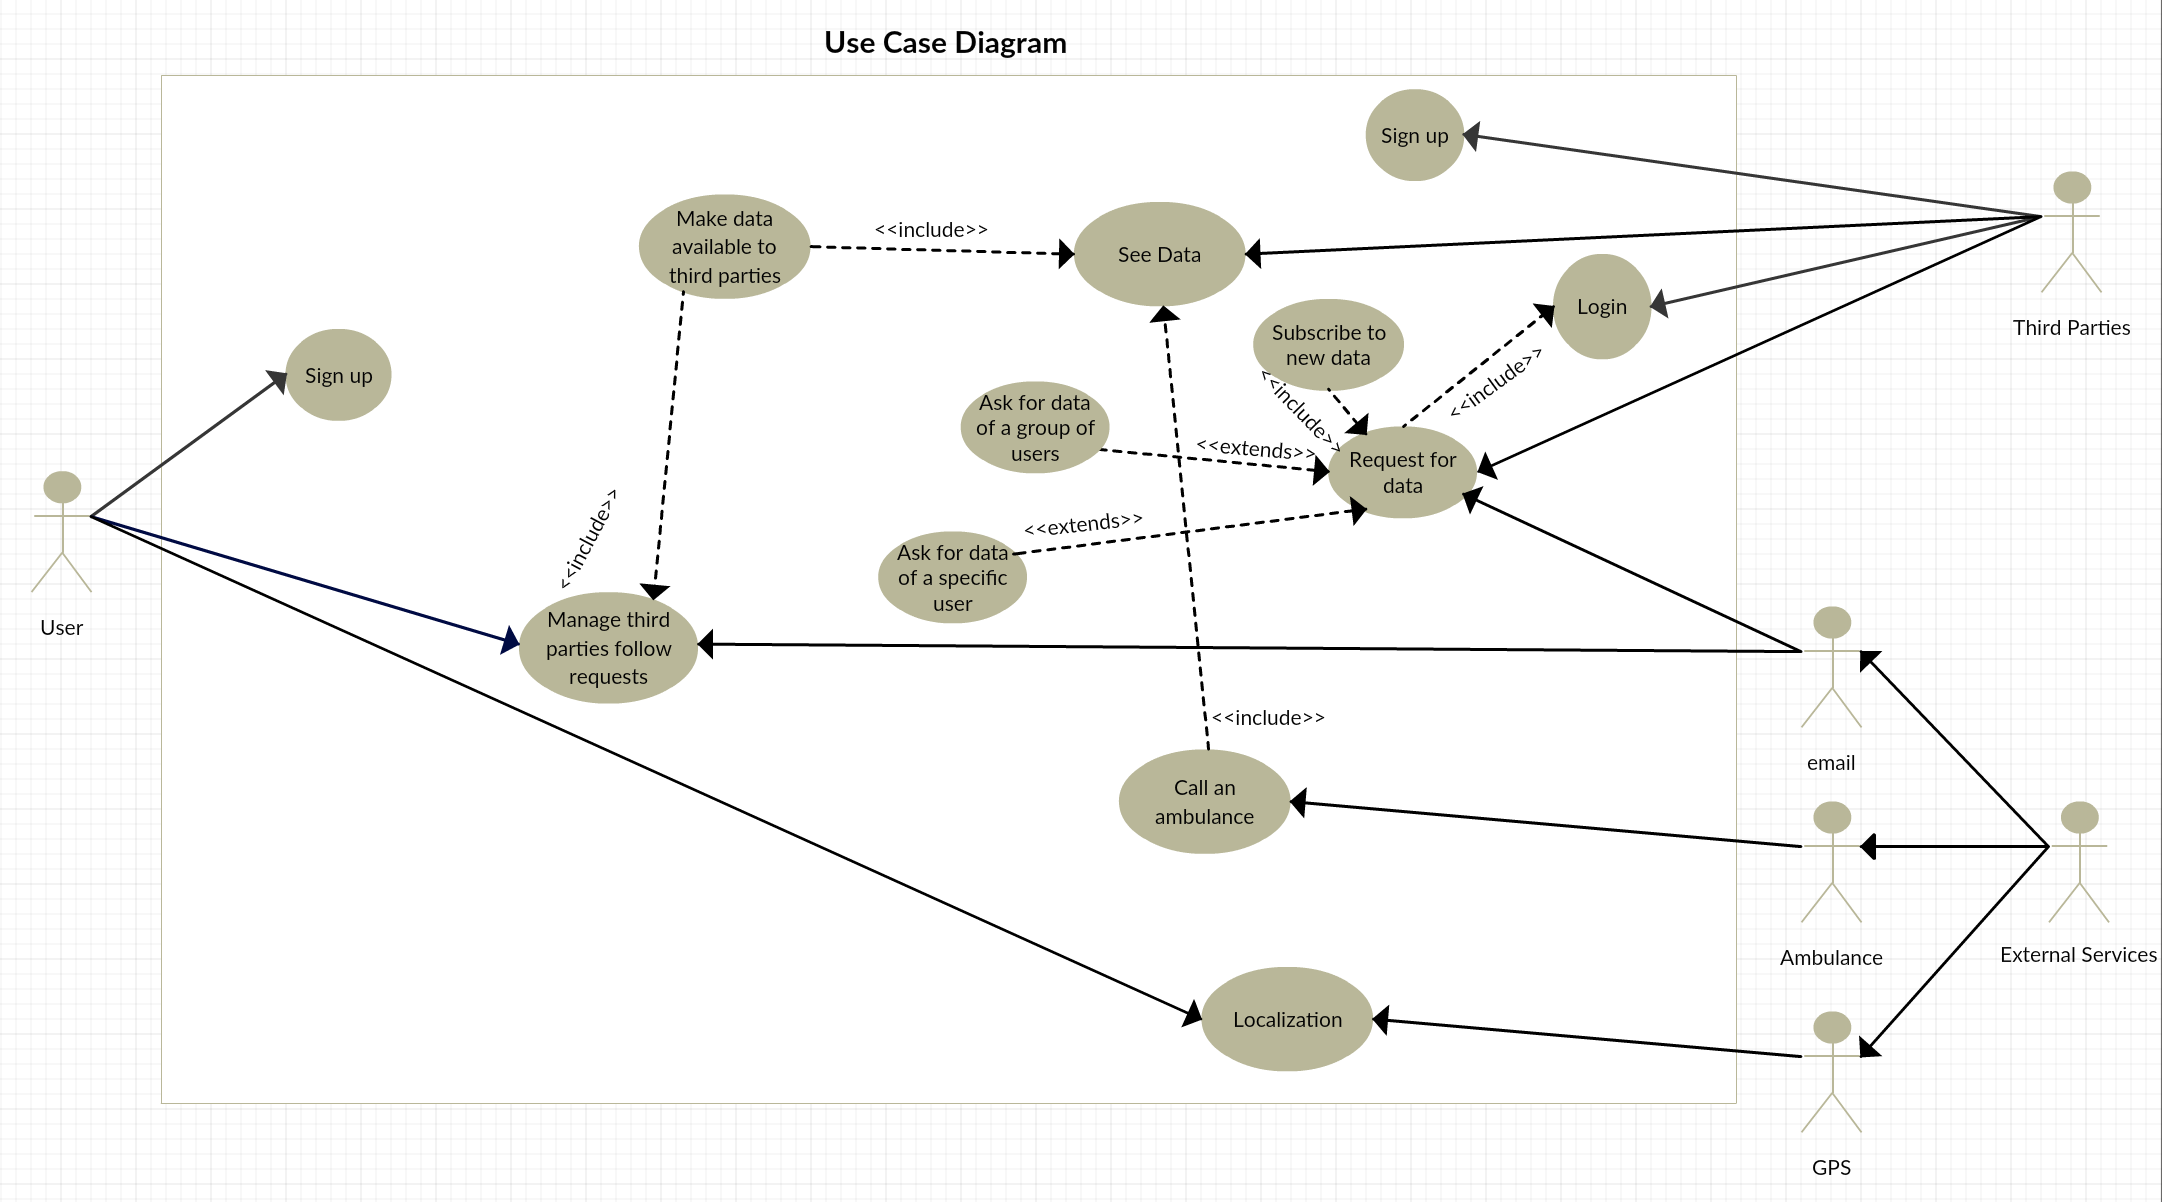
\includegraphics[width= \linewidth]{usecase.png}
\end{figure}
\begin{center}
    \begin{tabular}{ | l | p{10cm} |}
    \hline
    Name & Visitor sing up.\\ \hline
    Actors & User\\ \hline
   	Goals & {[G1]}\\ \hline
    Input Conditions & There are no entry conditions.\\ \hline
    Event Flow & \begin{enumerate}
    	\item The user on the web home page clicks on the sign in button to start the registration process.
    	\item The user insert his Google account or Apple account.
    	\item The user fills all the mandatory fills.
		\item The user clicks on the confirm button.
		\item The system saves the data.
    \end{enumerate} \\ \hline
    Output Conditions & The user successfully ends the registration process. From now on he can log into the application, providing his credentials and start using Data4Help. \\ \hline
    Exceptions & \begin{enumerate}
    	\item The user is already registered.
		\item The user inserts no valid information in one or more mandatory fills.
		\item The user chooses a username that has already been taken. 
		\item The user chooses an email that his associated with another user.
		\item The user chooses a Google account or Apple account that is already used.
	\end{enumerate}
All the exceptions are handled notifying the issues to the user and taking back the event flow to point 2.
    \\ \hline
    \end{tabular}
\end{center}

\begin{center}
    \begin{tabular}{ | l | p{10cm} |}
    \hline
    Name & User accept or reject third party requests.\\ \hline
    Actors & User\\ \hline
   	Goals & {[G2]}\\ \hline
    Input Conditions & The user receives a request of following.\\ \hline
    Event Flow & \begin{enumerate}
    	\item The user checks his email and open the following request.
		\item The user decides whether accepting it request or not, by clicking on one of the two button in the email.
    \end{enumerate} \\ \hline
    Output Conditions & The user is notified to have actually accepted/reject the request. TrackMe is notified that a request has been accepted/rejected. \\ \hline
    Exceptions & - \\ \hline
    \end{tabular}
\end{center}

\begin{center}
    \begin{tabular}{ | l | p{10cm} |}
    \hline
    Name & Third part sign up.\\ \hline
    Actors & Third part\\ \hline
   	Goals & {[G4]}\\ \hline
    Input Conditions & There are no entry conditions.\\ \hline
    Event Flow & \begin{enumerate}
    	\item The third part on the home page clicks on the sign in button to start the registration process.
		\item The third part fills all the mandatory fills.
		\item The third part clicks on the confirm button.
		\item The system saves the data.
    \end{enumerate} \\ \hline
    Output Conditions & The third part successfully ends the registration process. From now on it can log into the application, providing his credentials and start using Data4Help and AutomatedSOS.  \\ \hline
    Exceptions & \begin{enumerate}
    \item The third part is already registered.
	\item The third part inserts no valid information in one or more mandatory fills.
	\item The third part chooses a vat number that has already been taken. 
\end{enumerate} All the exceptions are handled notifying the issues to the third part and taking back the event flow to point 2.  \\ \hline
    \end{tabular}
\end{center}

\begin{center}
    \begin{tabular}{ | l | p{10cm} |}
    \hline
    Name & Third part login.\\ \hline
    Actors & Third part\\ \hline
   	Goals & {[G5]}\\ \hline
    Input Conditions & There third part is already in the homepage.\\ \hline
    Event Flow & \begin{enumerate}
    	\item The third part inserts its credentials in.
		\item The third part clicks on the login button in order to access.
		\item The system redirects the third part to his profile.
    \end{enumerate} \\ \hline
    Output Conditions & The third part his successfully redirects to his profile.  \\ \hline
    Exceptions & \begin{enumerate}
   \item The third part insert a not vat number.
	\item The third part insert a not valid password.
\end{enumerate} All the exceptions are handled notifying the issues to the user and taking back the event flow to point 1.    \\ \hline
    \end{tabular}
\end{center}

\begin{center}
    \begin{tabular}{ | l | p{10cm} |}
    \hline
    Name & Third part formulate a request to access anonymized data of a group of users.\\ \hline
    Actors & Third part\\ \hline
   	Goals & {[G6]}\\ \hline
    Input Conditions & The third part is already logged in into the system.\\ \hline
    Event Flow & \begin{enumerate}
    	\item The third part clicks on the \emph{group request}.
    	\item The request is filled using drop-down menu. Each drop-down menu is linked to a type of filter. By selecting a filter the company is able to better specify the composition of the group it is interested in.
		\item The request is sent to TrackMe by clicking on \emph{send} button. 
    \end{enumerate} \\ \hline
    Output Conditions & The request is sent to TrackMe and a message for the correct sending of the request is presented to the company. \\ \hline
    Exceptions & -   \\ \hline
    \end{tabular}
\end{center}

\begin{center}
    \begin{tabular}{ | l | p{10cm} |}
    \hline
    Name & Third part formulate a request to access data of a specific user through is SSN. \\ \hline
    Actors & Third part\\ \hline
   	Goals & {[G7]}\\ \hline
    Input Conditions & The third part is already logged in into the system.\\ \hline
    Event Flow & \begin{enumerate}
    	\item The third part clicks on the \emph{single user request}.
    	\item The request is filled with the user's SSN.
    	\item The request is sent to TrackMe by clicking on \emph{send} button. 
    \end{enumerate} \\ \hline
    Output Conditions & The request is sent to TrackMe and a message for the correct sending of the request is presented to the company.  \\ \hline
    Exceptions & -    \\ \hline
    \end{tabular}
\end{center}

\begin{center}
    \begin{tabular}{ | l | p{10cm} |}
    \hline
    Name & Third part can access anonymized data of a group of users.\\ \hline
    Actors & Third part\\ \hline
   	Goals & {[G8]}\\ \hline
    Input Conditions & There third part is already logged into the system.\\ \hline
    Event Flow & \begin{enumerate}
    	\item The third part accesses the approved group requests section.
		\item The third part selects an approved group request.
		\item The system redirects the third part to the request result.
    \end{enumerate} \\ \hline
    Output Conditions & The data requested by the third part are shown.  \\ \hline
    Exceptions & \begin{enumerate}
  		\item The data requested aren't anonymous since the outcome of the request concerns less than 1000 users.
\end{enumerate} All the exceptions are handled notifying the issues to the third part and taking back the event flow to point 1.    \\ \hline
    \end{tabular}
\end{center}

\begin{center}
    \begin{tabular}{ | l | p{10cm} |}
    \hline
    Name & Third part can access data of a specific user through his SSN.\\ \hline
    Actors & Third part\\ \hline
   	Goals & {[G9]}\\ \hline
    Input Conditions & There third part is already logged into the system.\\ \hline
    Event Flow & \begin{enumerate}
    	\item The third part accesses the approved single user requests section.
    	\item The third part selects an approved single user request. 
    	\item The system redirects the third part to the request result.
    \end{enumerate} \\ \hline
    Output Conditions & The data requested by the third part are shown.  \\ \hline
    Exceptions & \begin{enumerate}
   \item The user didn't approve the request.
\end{enumerate} All the exceptions are handled notifying the issues to the third part and taking back the event flow to point 1.    \\ \hline
    \end{tabular}
\end{center}

\begin{center}
    \begin{tabular}{ | l | p{10cm} |}
    \hline
    Name & Data4Help can anonymise data. \\ \hline
    Actors & TrackMe\\ \hline
   	Goals & {[G11]}\\ \hline
    Input Conditions & Third part has requested data of a group of users.\\ \hline
    Event Flow & \begin{enumerate}
		\item TrackMe performs the research among the matching users.
		\item TrackMe anonymize the data of the selected users.
    \end{enumerate} \\ \hline
    Output Conditions & The data requested from the third part are anonymized. \\ \hline
    Exceptions & \begin{enumerate}
  		\item The data requested aren’t anonymous since the outcome of the request concerns less than 1000 users.
\end{enumerate} All the exceptions are handled notifying the issues to the third part and taking back the event flow to point 1.    \\ \hline
    \end{tabular}
\end{center}

\begin{center}
    \begin{tabular}{ | l | p{10cm} |}
    \hline
    Name & TrackMe can forward third parties requests to users. \\ \hline
    Actors & TrackMe\\ \hline
   	Goals & {[G12]}\\ \hline
    Input Conditions & Third part has requested data of a single user.\\ \hline
    Event Flow & \begin{enumerate}
    	\item TrackMe forwards the request of being observed by a specific company to the user.
    	\item TrackMe marks the user as \emph{pendent user}.
    \end{enumerate} \\ \hline
    Output Conditions & The request of being followed by a company is sent to the user. \\ \hline
    Exceptions & -    \\ \hline
    \end{tabular}
\end{center}\newpage

\subsubsection{Sequence diagram}

\begin{figure}[h!]
\centering
    \textbf{Company formulate single user request.}\par\medskip
	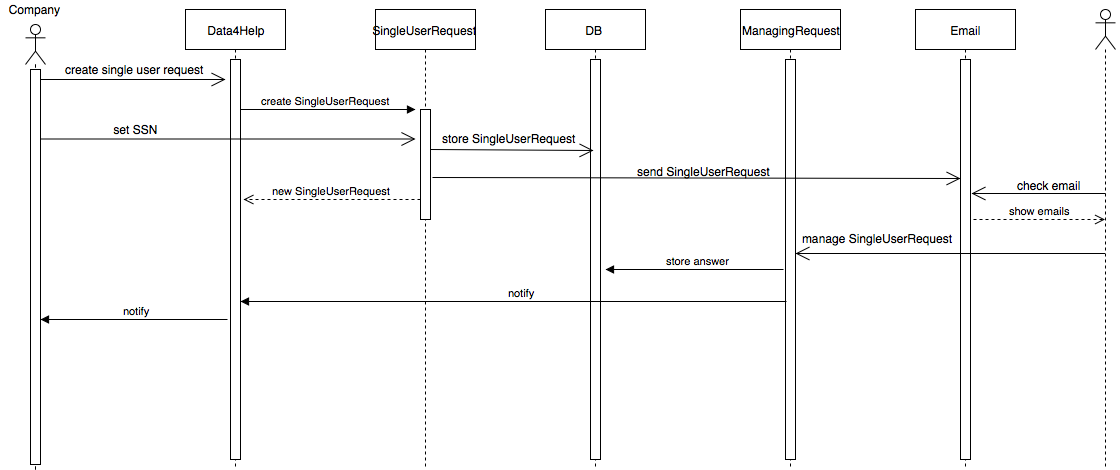
\includegraphics[width= \linewidth]{singlerequest.png}
\end{figure}\newpage
\begin{figure}[h!]
\centering
    \textbf{Company formulate group user request.}\par\medskip
	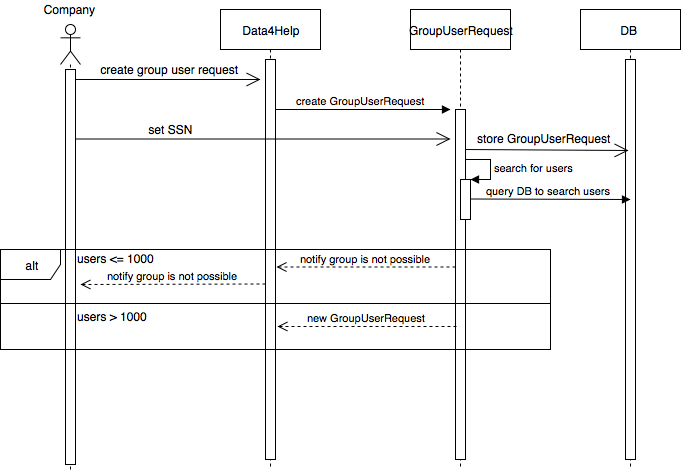
\includegraphics[width= \linewidth]{grouprequest.png}
\end{figure}\newpage
\begin{figure}[h!]
\centering
    \textbf{User accept or reject a following request.}\par\medskip
	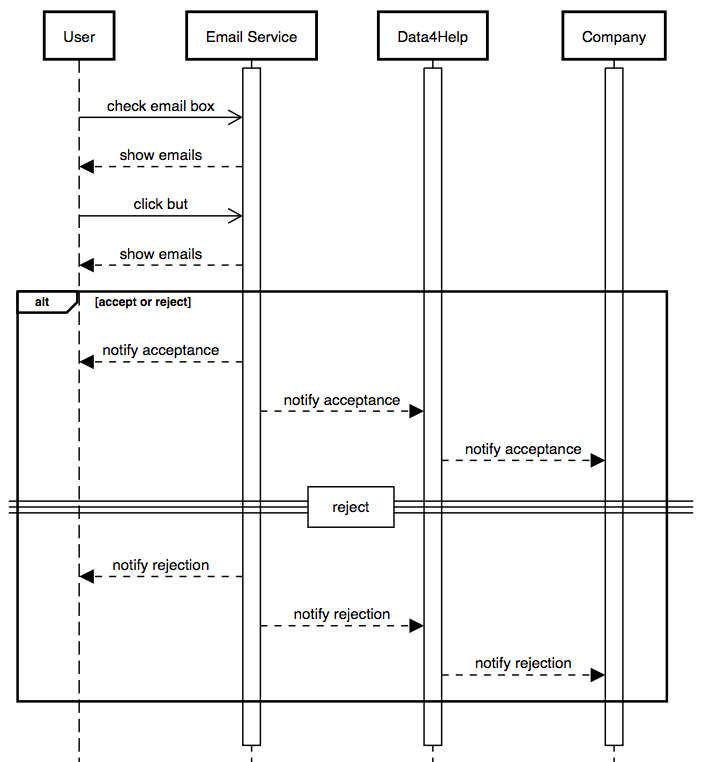
\includegraphics[width= \linewidth]{acceptreject.png}
\end{figure}\newpage
\begin{figure}[h!]
\centering
    \textbf{AutomatedSOS calls an ambulance.}\par\medskip
	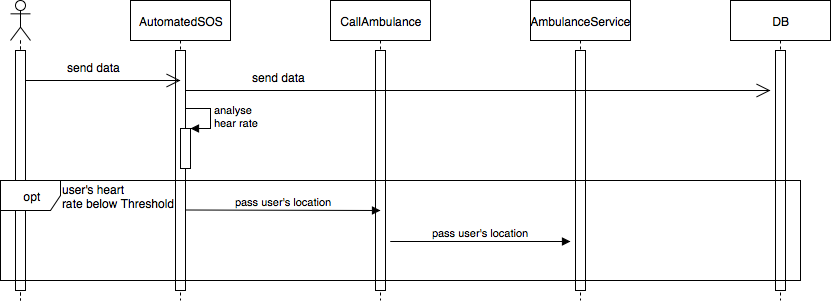
\includegraphics[width= \linewidth]{callambulance.png}
\end{figure}\newpage
\subsection{Performance requirements}
\begin{itemize}
	\item AutomatedSOS calls an ambulance to the current user's position within 5 seconds.
\end{itemize}
\subsection{Design constraints}
\subsubsection{Standard compliance}
\subsubsection{Hardware limitation}
\subsubsection{Other constraints}
\subsection{Software system attributes}
\subsubsection{Reliability}
\subsubsection{Security}
\subsubsection{Maintainability}
\subsubsection{Compatibility}
\section{Formal Analysis Using Alloy}
\subsection{Alloy model}
\subsection{World generated}
\subsection{Alloy results}
\section{Effort Spent}
\section{Resources}
\end{document}


